\documentclass{article}
\usepackage{algorithm}
\usepackage{algorithmic}
\usepackage{amsmath}
\usepackage{amssymb}
\usepackage{booktabs}
\usepackage{caption}
\usepackage{CJKutf8}
%\usepackage{ctex}  %使用宏包(为了能够显示汉字)
%\usepackage{CJK}
\usepackage{diagbox}	%斜线表头
\usepackage{float}
\usepackage{geometry}
\usepackage{graphicx}
\usepackage{ulem}
\usepackage{geometry}
\usepackage{graphicx}
\usepackage{hyperref}
\usepackage{listings}
\usepackage{setspace}%行间距
\usepackage{subfigure}%并排子图 共享标题 有子标题
\usepackage{textcomp}
\usepackage{url}
\usepackage{verbatim}%多行注释
\usepackage{xcolor}
%\usepackage{fontspec}
%\setmonofont{Consolas}
\linespread{2.0}


%\tiny
%\scriptsize
%\footnotesize
%\small
%\normalsize
%\large
%\Large
%\LARGE
%\huge
%\Huge

\geometry{a4paper, left = 1.5cm, right = 1.5cm, top = 1cm, bottom = 2cm}
\lstset{
    backgroundcolor=\color{red!5!green!5!blue!5},%代码块背景色为浅灰色
    rulesepcolor= \color{gray}, %代码块边框颜色
    breaklines=true,  %代码过长则换行
    numbers=left, %行号在左侧显示
    numberstyle= \small,%行号字体
    keywordstyle= \color{red},%关键字颜色
    commentstyle=\color{gray}, %注释颜色
    frame=shadowbox,%用方框框住代码块
    escapeinside=``%逃逸字符,用于在插入代码中输入中文
    }

%%%%%%%%%%%%%%%%%%%%%%%%%%%%%%%%%%%%%%%%%%%%%%%%%%%%%%%%%%%%%%%%%%%%%%%%%%%
\begin{document}
	\title{Report on HttpComponents}  %———总标题
	\begin{center}
		\huge Report on Httpcomponents\\
		\hspace*{\fill} \\ %空行
		\begin{CJK}{UTF8}{gbsn}
			\normalsize 张宇轩, 2017K8009908041\\
		\end{CJK}{}
	\end{center}
	\begin{figure}[H]
		\centering
		
\includegraphics[height = 3.5cm, width = 5.5cm]{pics/1_httpcomponents.png}	
		%\caption{}
	\end{figure}

	\hspace*{\fill} \\ %空行
	
	\tableofcontents{} %—— 制作目录(目录是根据标题自动生成的)
	\clearpage
%%%%%%%%%%%%%%%%%%%%%%%%%%%%%%%%%% NEW PAGE %%%%%%%%%%%%%%%%%%%%%%%%%%%%%%%%%%%%%%%%%
	\section{Preface}
	\subparagraph{}
	\begin{CJK}{UTF8}{gbsn}
		由于先前的课程中并没有讲过关于网络与信息方面的知识,笔者之也并没有接触过。而这次的选题是HttpComponents,涉及到大量的网络方面的知识,所以在准备这篇报告的第一阶段笔者的主要精力是放在研究一些基本的网络方面的知识。要讲到HttpComponents,就先要讲一下关于http的各种知识。
	\end{CJK}{}
	\clearpage
	
	\begin{comment}
	\paragraph{}
	\indent \indent 
	\begin{CJK}{UTF8}{gbsn}
		第一阶段解读的重点放在了连接http周边知识上。  
	\end{CJK}{}
	\end{comment}

	\section{Related Introduction}

	\subsection{http}
	\subparagraph{}
	%\indent \indent 
	\begin{CJK}{UTF8}{gbsn}
		从万维网(World Wide Web )服务器传输超文本到本地浏览器,基于请求与响应,无状态的,应用层的协议。
从本地角度去看http协议,就相当于浏览器访问一个url,然后就得到相应的web页面
从服务器角度去看http协议,就相当于客户端(浏览器)链接远程http服务器,服务器返回数据,浏览器接收、解析数据之后显示出来。 
	\end{CJK}{}
	\subsection{https}
	\subparagraph{}
	%\indent \indent 
	\begin{CJK}{UTF8}{gbsn}
		利用SSL(此处:基于应用层的访问控制)进行传输层加密的http传输协议,更加安全。\\ 
		https = http + SSL
	\end{CJK}{}
	\subsection{Proxy Server}
	\subparagraph{}
	\begin{CJK}{UTF8}{gbsn}
		代理服务器:代理个人网络从互联网服务商那里获取信息(通过在二者间建立非直接的连接),可以保证安全。
	\end{CJK}{}
	\subsection{Cookies}
	\subparagraph{}
	\begin{CJK}{UTF8}{gbsn}
		网站保存在用户端的含有用户信息以及行为的文本,用以弥补http协议的无状态性。举两个例子:
	\end{CJK}{}

	%\begin{comment}
	\begin{center}
	\fbox{
		\shortstack[l]{
	    	\begin{CJK}{UTF8}{gbsn}
				1.网站上的记住密码。网站将用户的身份和密码经过加密cookies存在用户硬盘中,下次登录的时候就不用手动输密码了。
			\end{CJK}{}\\
			\begin{CJK}{UTF8}{gbsn}
				2.上下文相关网址。如果上一个页面会对下一个页面产生影响,那次是就必须使用cookies。
			\end{CJK}{}\\
			\begin{CJK}{UTF8}{gbsn}
				比如一个购物网站,上一个页面选好商品,接下来的页面进行支付,支付页面就必须知道上一个页面中购买了什么东西,
			\end{CJK}{}\\
			\begin{CJK}{UTF8}{gbsn}
				此时就需要cookies。
			\end{CJK}{}
		}
	}
	\end{center}
	%\end{comment}

	\subsection{Request Format}
	\subparagraph{}
	\begin{CJK}{UTF8}{gbsn}
		客户端发送一个请求到服务器的请求消息格式如 Figure 1 所示(后面还会说到),请求头部的最后会有一个空行,表示请求头部结束,接下来为请求数据。
	\end{CJK}{}

	\begin{figure}[H]
		\centering
		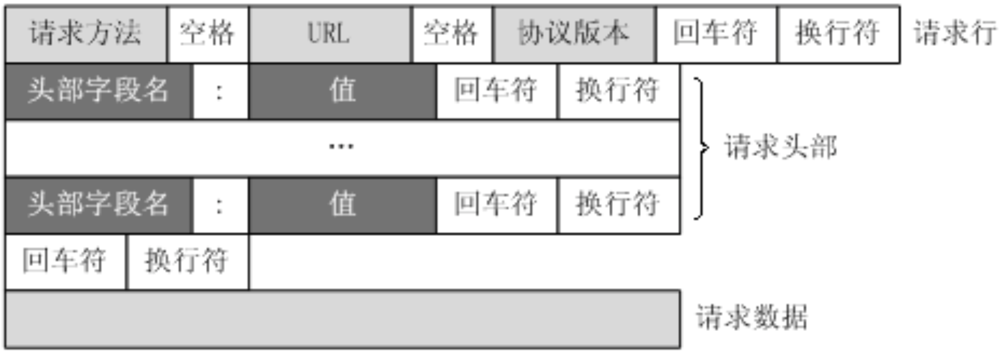
\includegraphics[height = 4.5cm, width = 12cm]{pics/2_request_format.png}	
		\caption{Request Format}
	\end{figure}
	\subsection{URL}
	\subparagraph{}
	\begin{CJK}{UTF8}{gbsn}
		URL(Uniform Resource Locator,统一资源定位符):一种资源位置的抽象唯一识别方法。\\
		URL组成:$<$协议$>$://$<$主机$>$:$<$端口$>$/$<$路径$>$ (端口和路径可以省略,端口默认80),如 Figure 2 所示: \\
		另外需要注意URI(Uniform Resource Identifier,统一资源标识符),用来表示web上每一种可用的资源,与URL不一样。 
	\end{CJK}{}
	\begin{figure}[H]
		\centering
		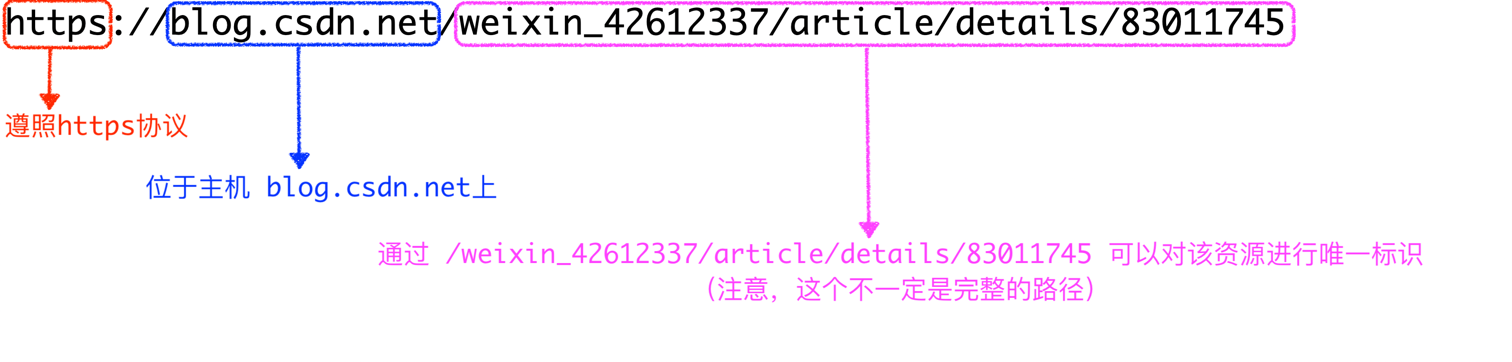
\includegraphics[height = 3.5cm, width = 16cm]{pics/3_url.png}	
		\caption{Request Format}
	\end{figure}

	\subsection{Http Request Methods}
	\subparagraph{}
	\begin{CJK}{UTF8}{gbsn}
		Http 协议共有9种请求方法,如 Figure 3 所示,其中最常用的两种方法是 GET 和 POST,其对比如 Figure 4 所示。\\
		GET - 从指定的资源请求数据。\\
		POST - 向指定的资源提交要被处理的数据。
	\end{CJK}{}
	\begin{figure}[H]
		\centering
		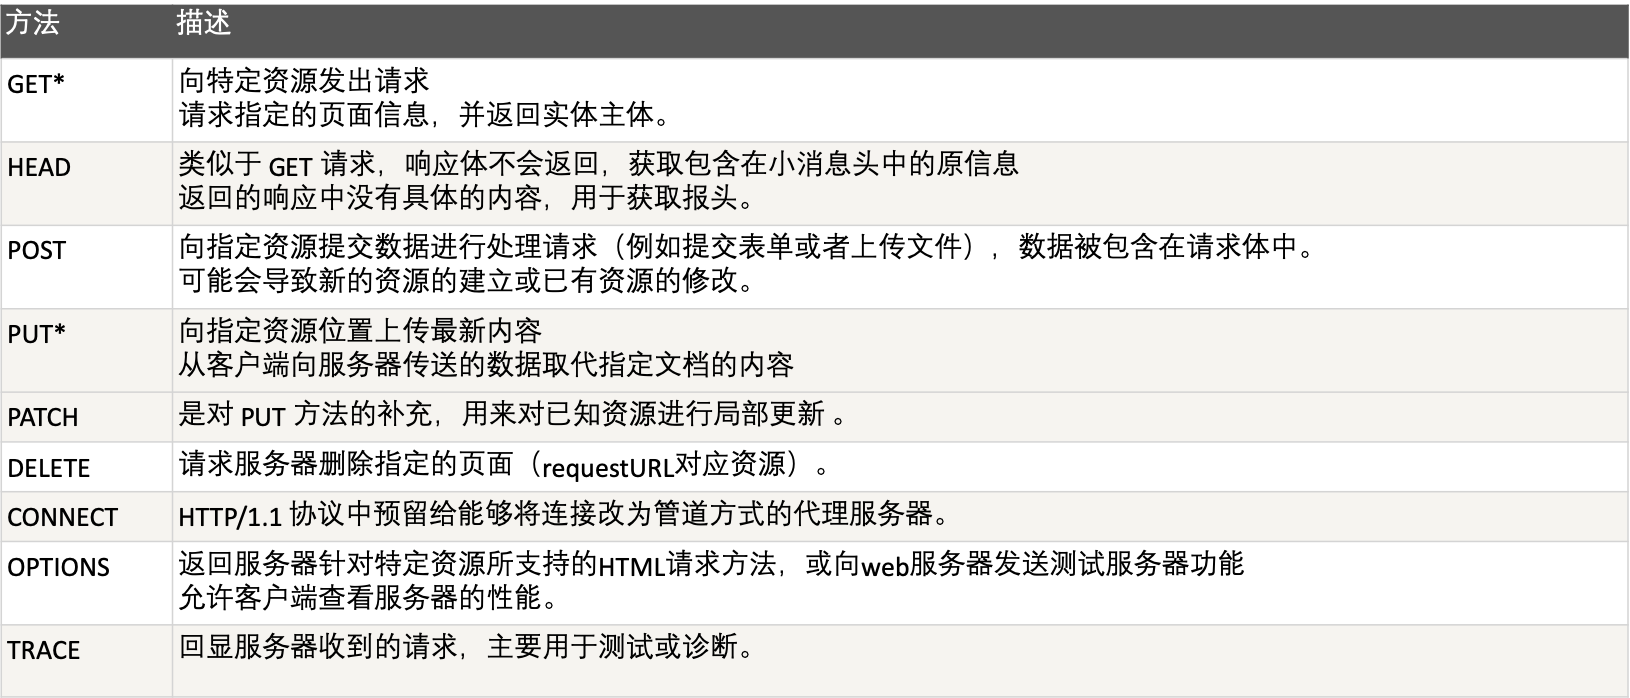
\includegraphics[height = 7.6cm, width = 16cm]{pics/4_9ways_of_http_request.png}	
		\caption{Request Format}
	\end{figure}
	\begin{figure}[H]
		\centering
		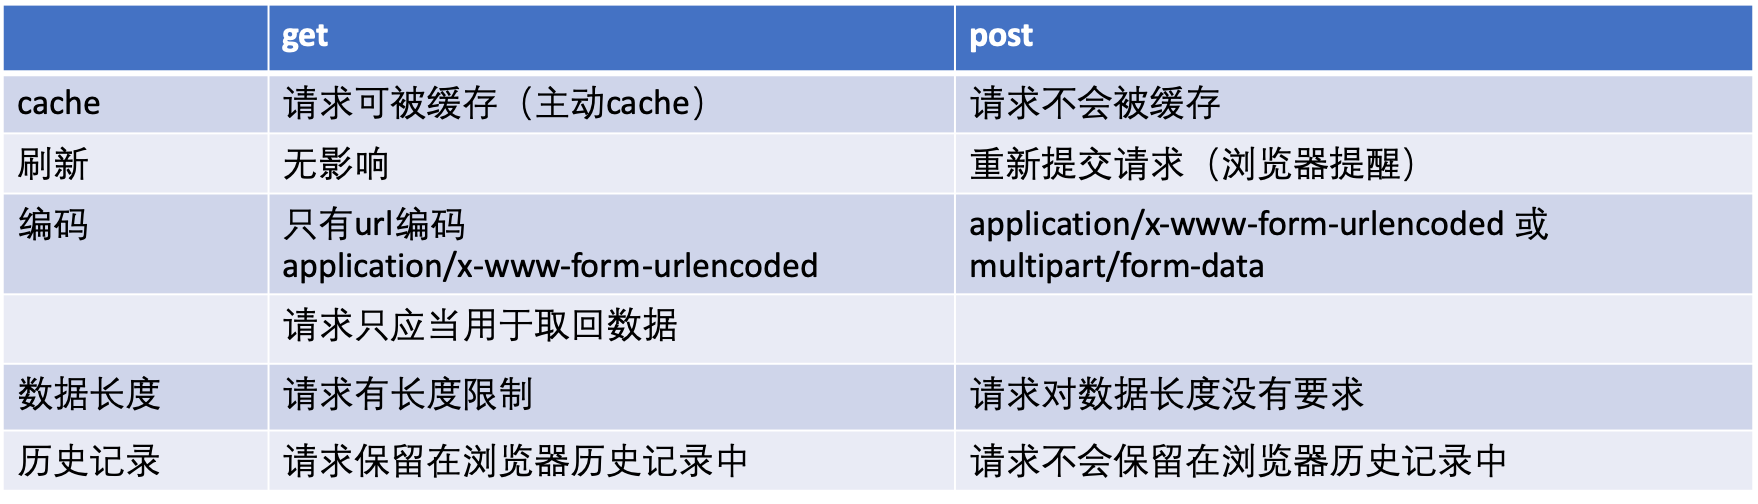
\includegraphics[height = 4.8cm, width = 15cm]{pics/5_get_post.png}	
		\caption{Get and Post}
	\end{figure}
	\begin{CJK}{UTF8}{gbsn}
		本文要介绍的HttpComponents就是用于提供对于http服务器的访问功能。
	\end{CJK}{}
	\section{About HttpComponents}
	%\subparagraph{}
	\begin{CJK}{UTF8}{gbsn}
		\subparagraph{}
		HttpComponents:用于提供对于http服务器的访问功能的超文本传输协议,其对HTTP底层协议进行了很好的封装。
		\subparagraph{}
		在构建HTTP客户端或者服务器端应用中很常见,比如WEB浏览器、爬虫、HTTP代理、WEB服务库、基于调整或扩展HTTP协议的分布式通信系统 etc.  
	\end{CJK}{}
	\subsection{Major Function}
	\begin{CJK}{UTF8}{gbsn}
		实现http方法:GET, HEAD, POST, PUT, DELETE, CONNECT, OPTIONS, TRACE, PATCH\\
		对https协议的支持(https = http + SSL)\\
		对代理服务器的支持\\
		对cookies的支持\\
		支持在特定的执行上下文(HTTP上下文)中执行HTTP消息——http不行( 无状态、面向响应请求 ) \\
	\end{CJK}{}
	\subsection{Component Structure}
	\begin{CJK}{UTF8}{gbsn}
		HttpComponents 的组件结构如 Figure 5 所示,包含 HttpComponents Core 和 HttpComponents AsyncClient,本次分析的是 HttpComponents Core。\\
	\end{CJK}{}
	\begin{figure}[H]
		\centering
		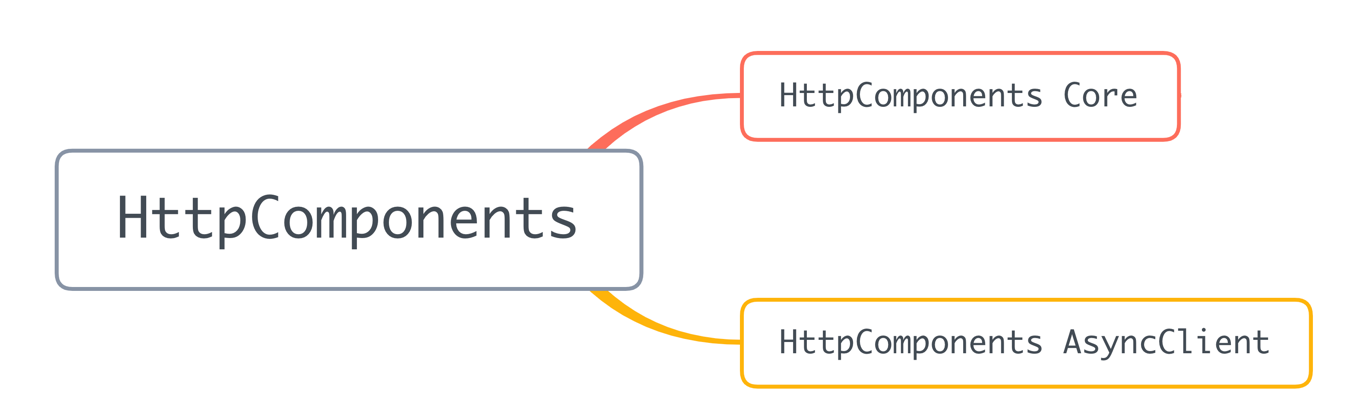
\includegraphics[height = 4cm, width = 12cm]{pics/6_httpcomponents_structure.png}	
		\caption{Component Structure of HttpsComponents}
	\end{figure}
	\subsection{HttpComponents Core}
	\begin{CJK}{UTF8}{gbsn}
		\subparagraph{}
		HttpComponents Core 简称 HttpCore,其实现基本http协议的组件,用于搭建客户端和服务器端的http服务。\\
		HttpCore 希望在实现基本的http功能的基础上提高性能与平衡性,如 Figure 6 所示:\\
		\begin{figure}[H]
		\centering
		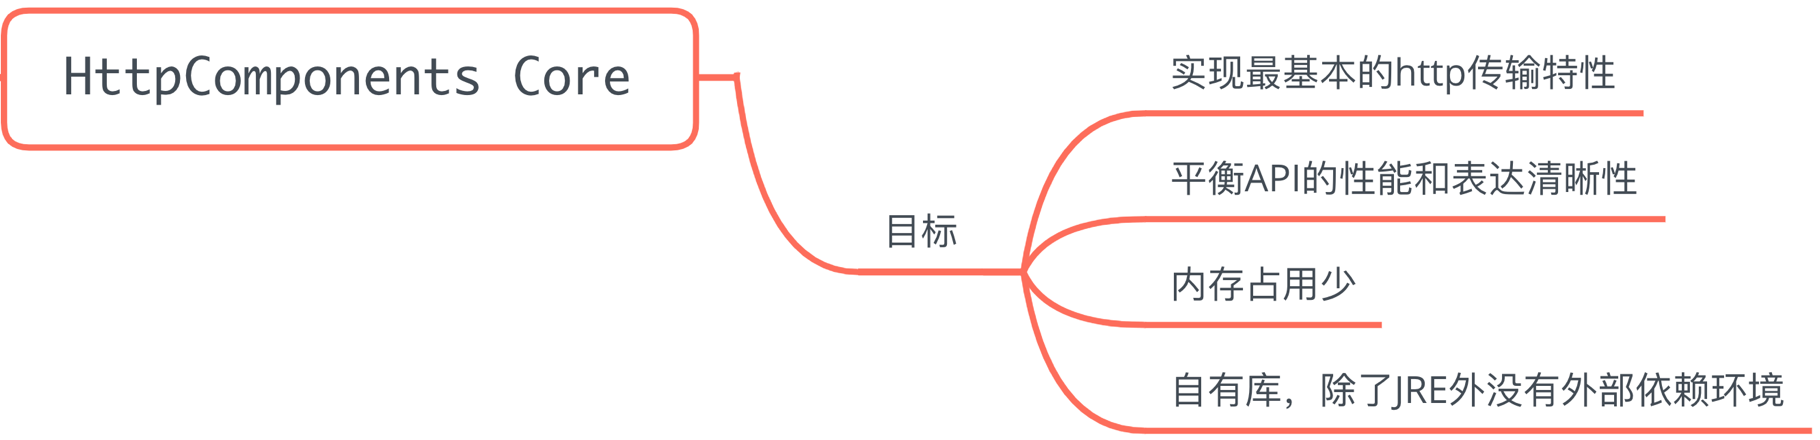
\includegraphics[height = 4cm, width = 16cm]{pics/9_target.png}	
		\caption{Goal of HttpCore}
		\end{figure}
		\begin{figure}[H]
		%\hspace*{\fill} \\ %空行
		\centering
		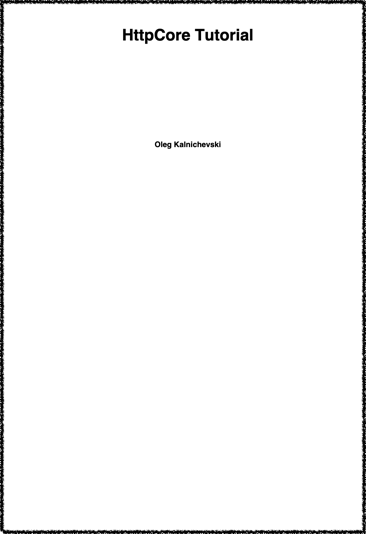
\includegraphics[height = 10cm, width = 7.5cm]{pics/7_guide_book.png}	
		\caption{Guide Book}
		\end{figure}
		官方文档: httpcore-tutorial http://hc.apache.org/httpcomponents-core-ga/tutorial/pdf/httpcore-tutorial.pdf
	\end{CJK}{}
	\subsubsection{Contents of HttpCore}
	\begin{CJK}{UTF8}{gbsn}
		\subparagraph{}
		HttpCore 共有 241 个类,如 Figure 8 所示。其中将会重点介绍 BasicHttpRequest 和 BasicHttpResponse 这两个类。\\
 	\end{CJK}{}
	\begin{figure}[htbp]
		\centering
		\subfigure[]{
			\begin{minipage}[t]{0.45\linewidth}
				\centering
				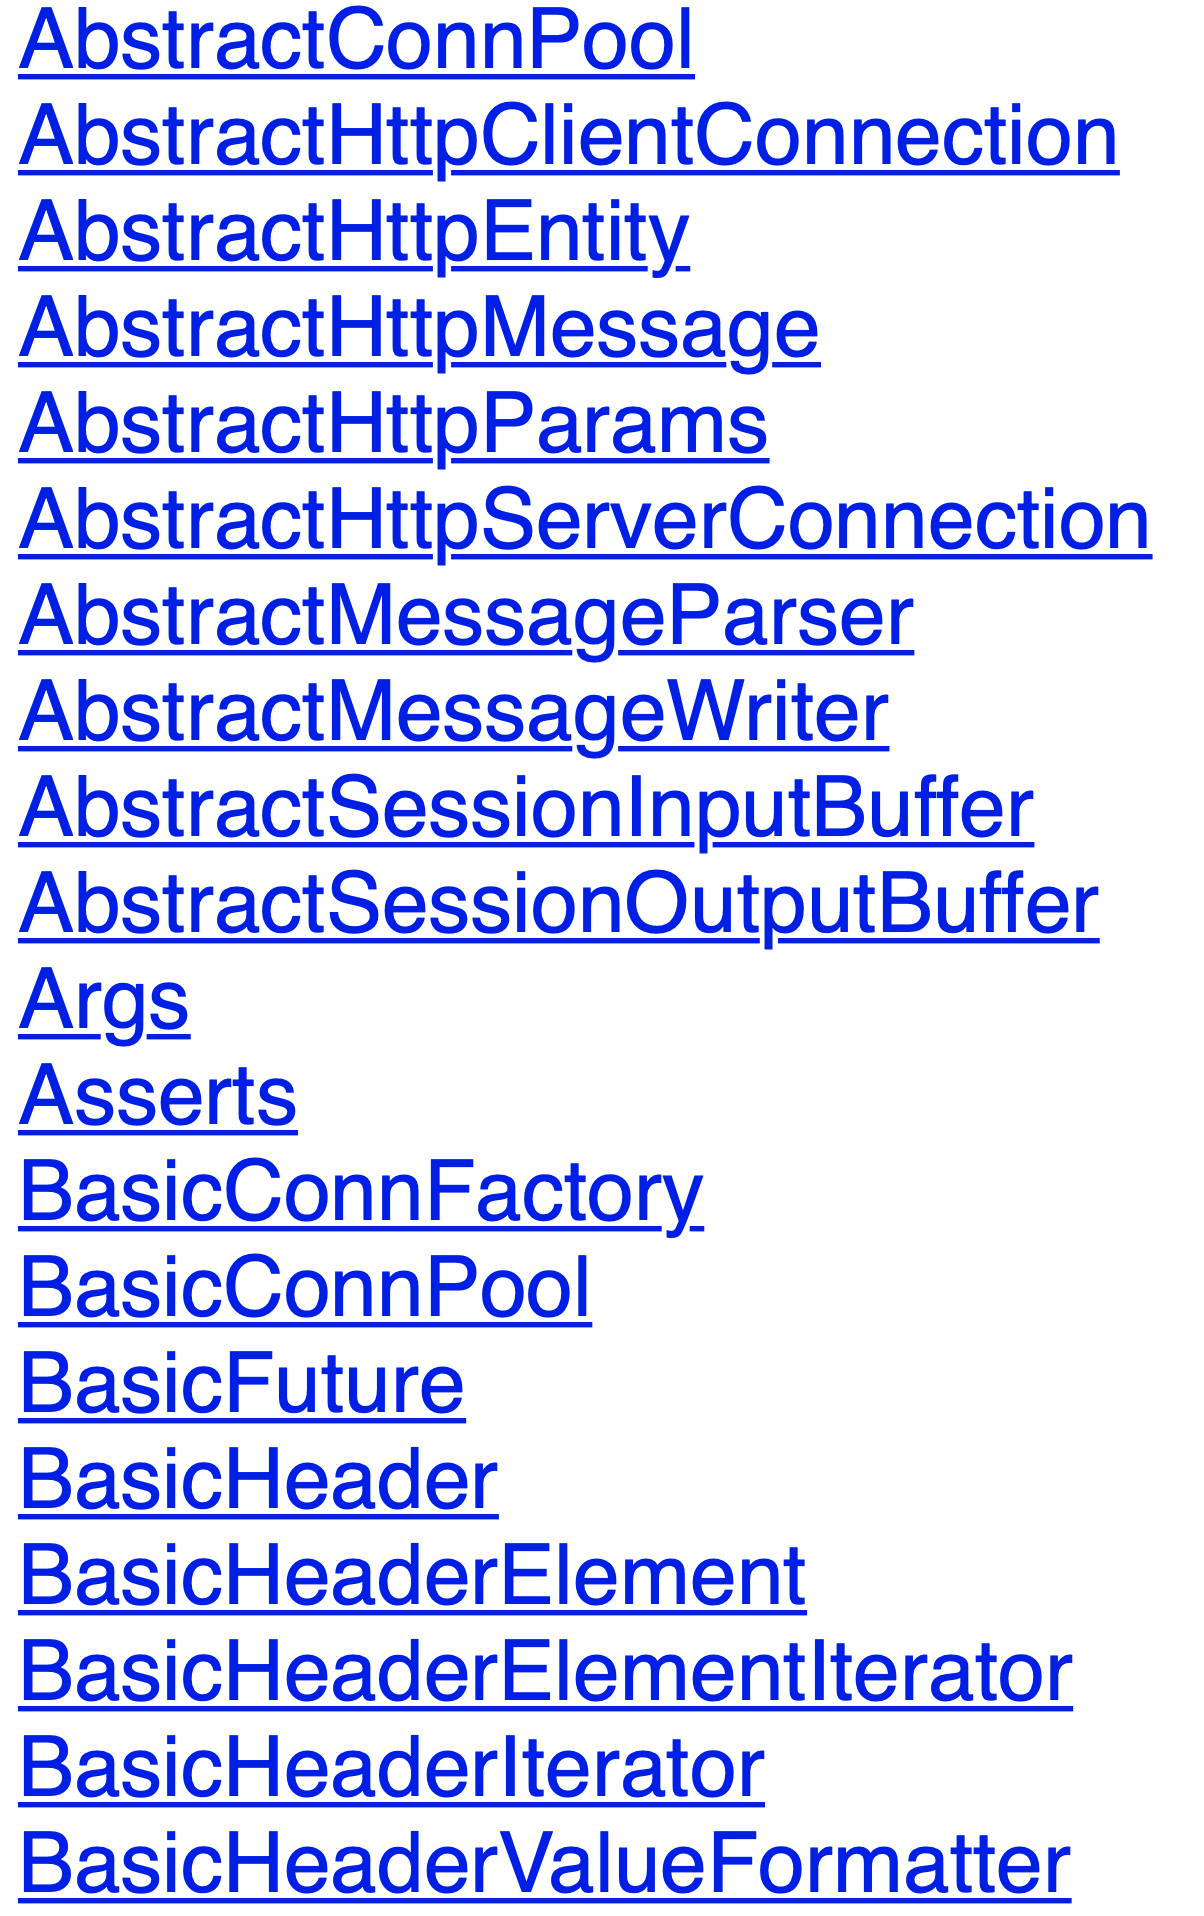
\includegraphics[width = 1in]{pics/11_all_classes.png}
				%\caption{fig1}
			\end{minipage}%
		}
		\subfigure[]{
			\begin{minipage}[t]{0.45\linewidth}
				\centering
				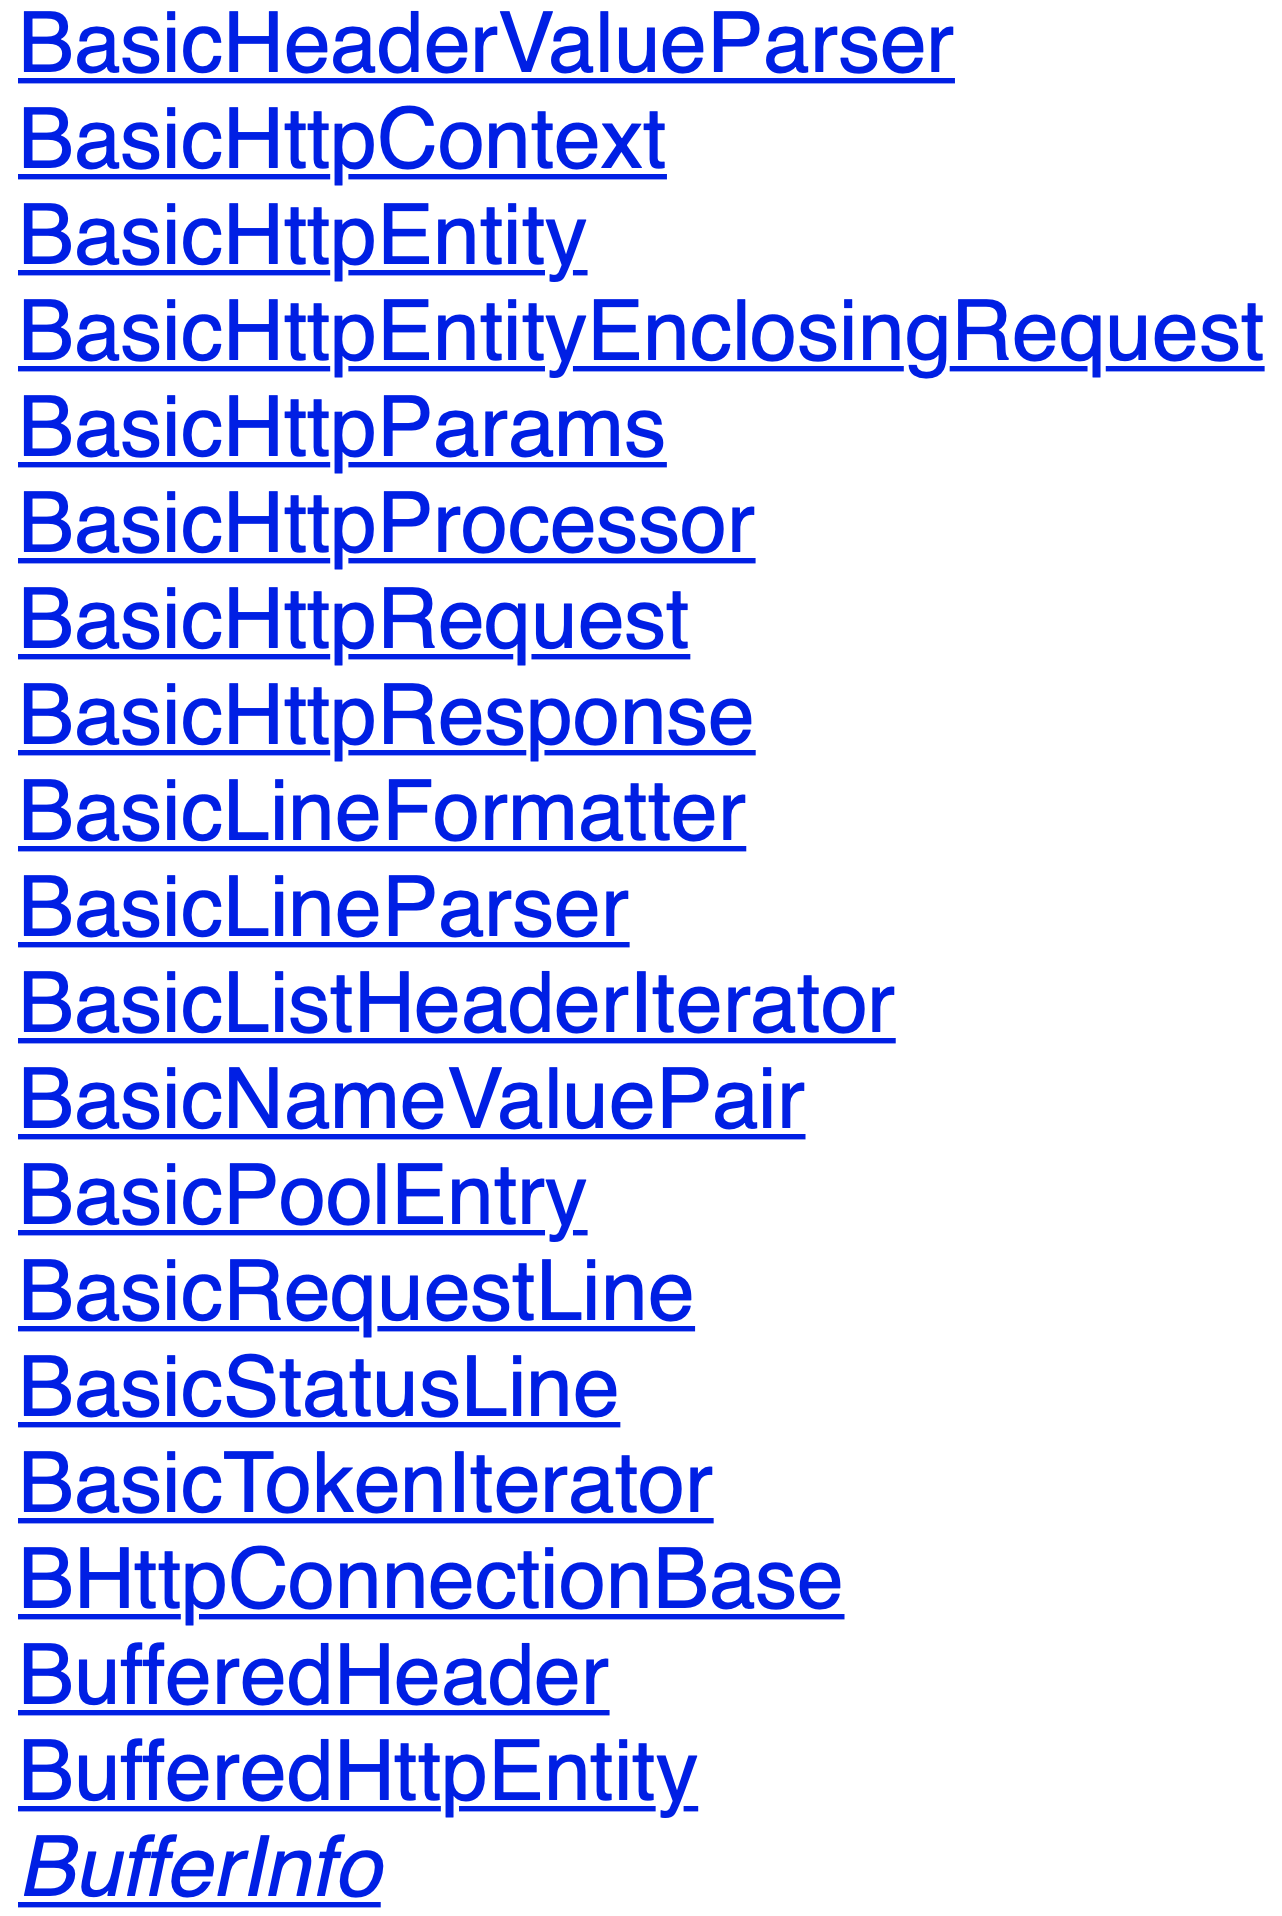
\includegraphics[width = 1in]{pics/12_all_classes.png}
				%\caption{fig2}
			\end{minipage}%
		}%
		\quad
		\subfigure[]{
			\begin{minipage}[t]{0.45\linewidth}
				\centering
				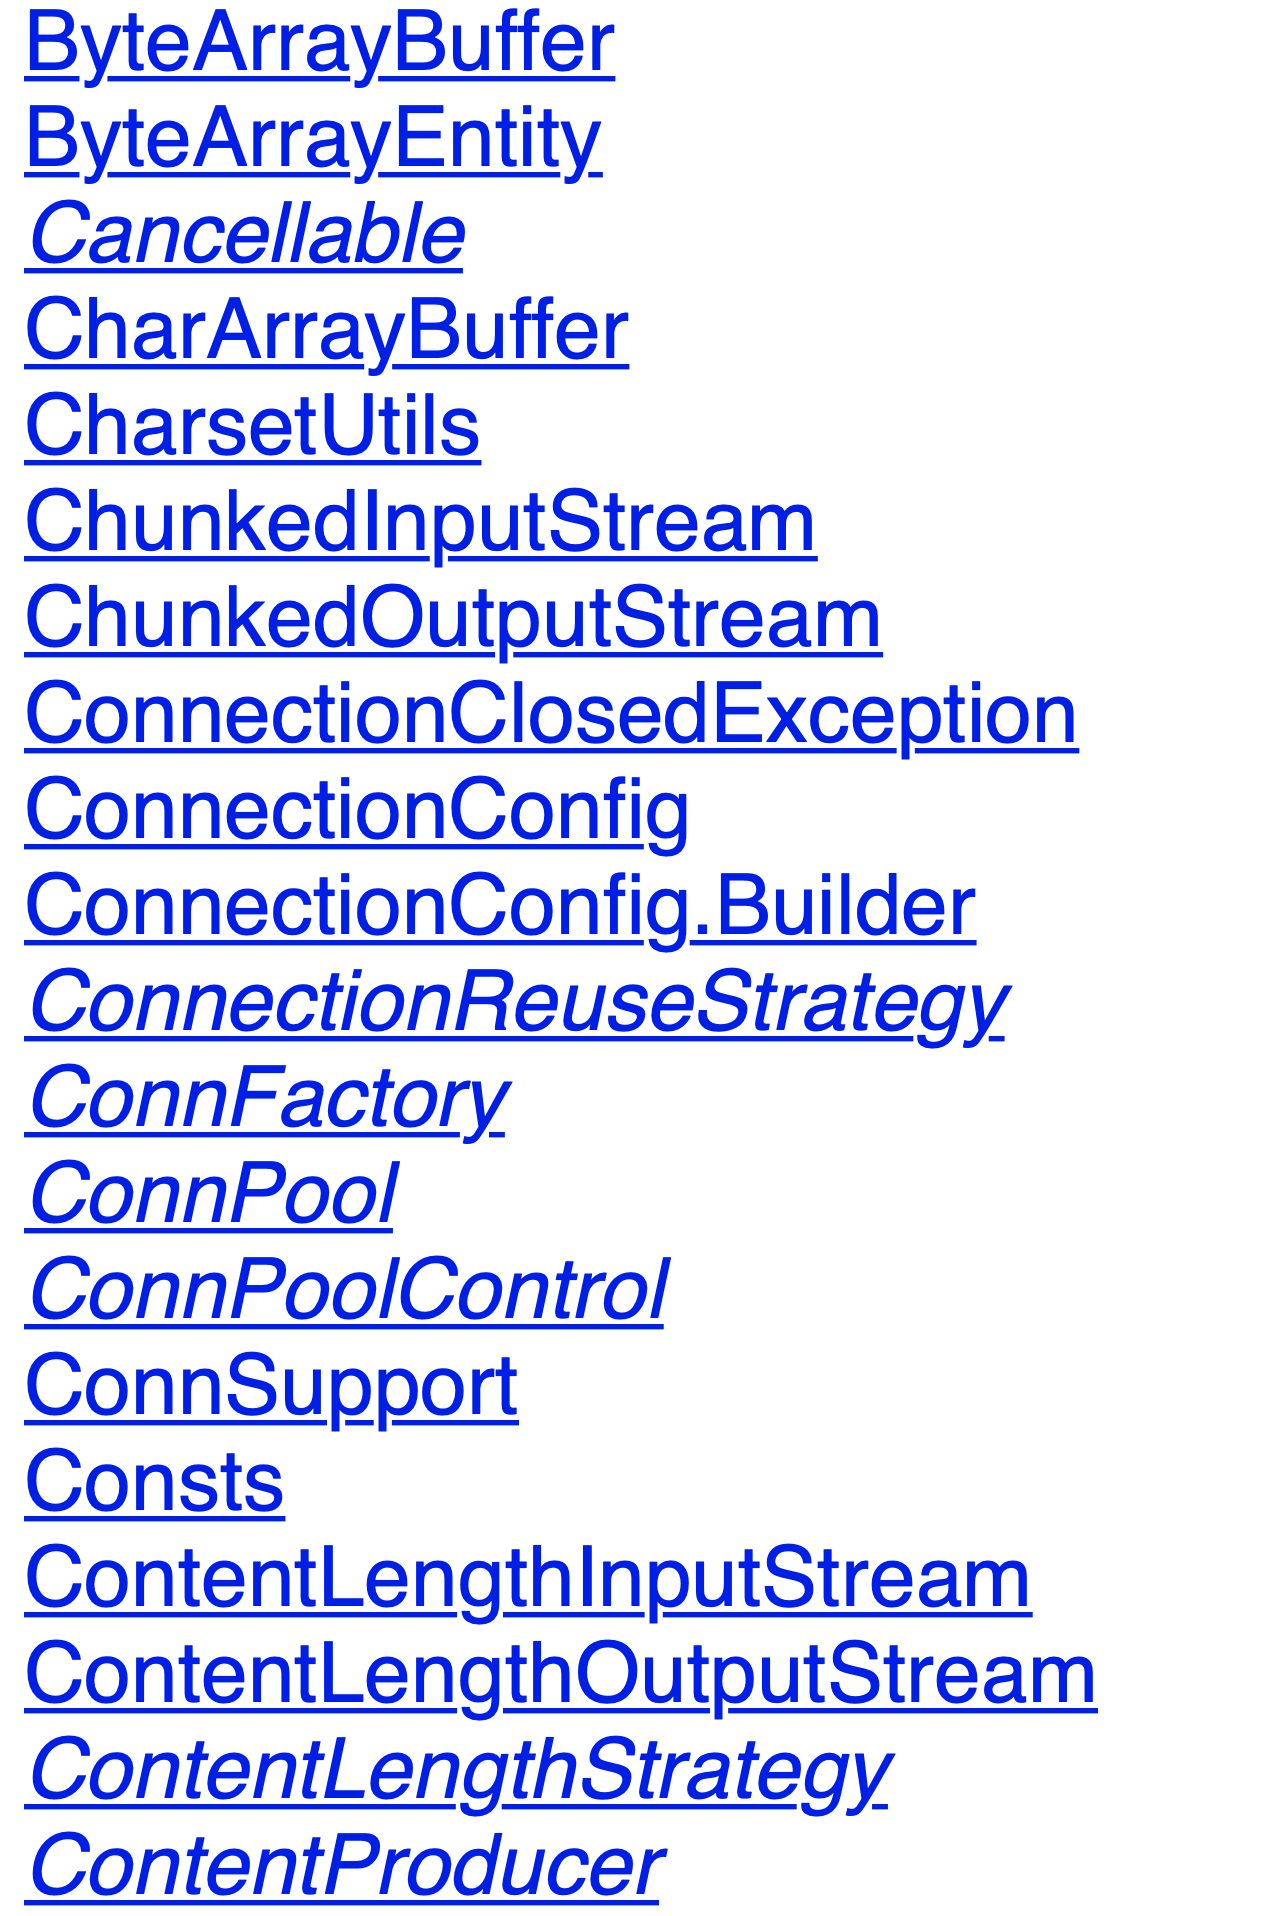
\includegraphics[width = 1in]{pics/13_all_classes.png}
				%\caption{fig2}
			\end{minipage}
		}%
		\subfigure[]{
			\begin{minipage}[t]{0.45\linewidth}
				\centering
				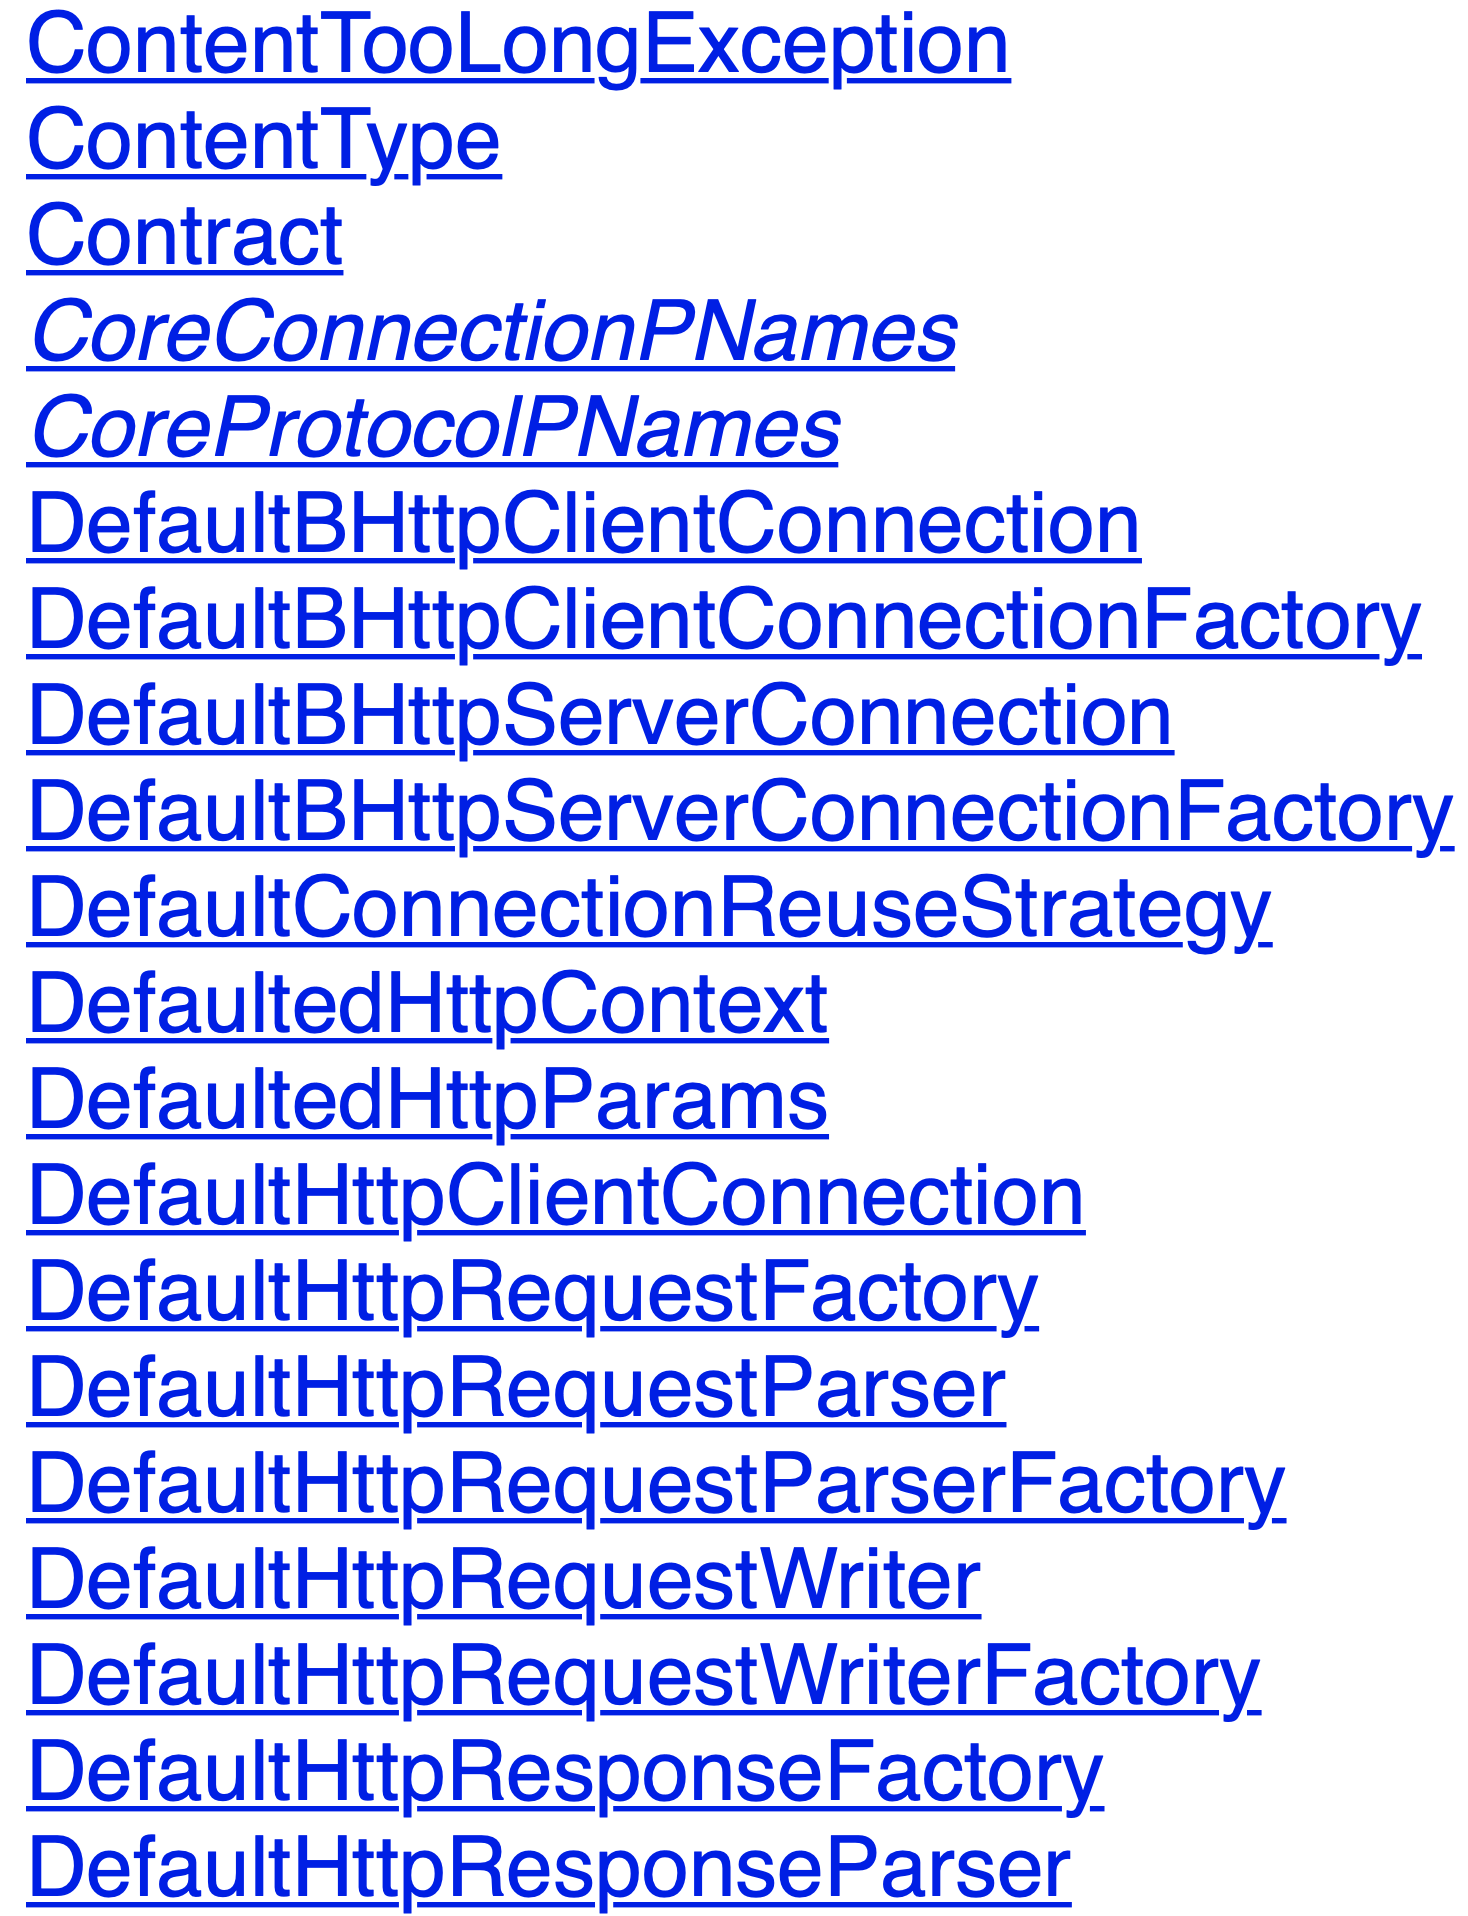
\includegraphics[width = 1in]{pics/14_all_classes.png}
				%\caption{fig2}
			\end{minipage}
		}%
		
		\centering
		%\caption{ pics}
	\end{figure}
	\clearpage

	\begin{figure}[htbp]
		\centering
		\subfigure[]{
			\begin{minipage}[t]{0.45\linewidth}
				\centering
				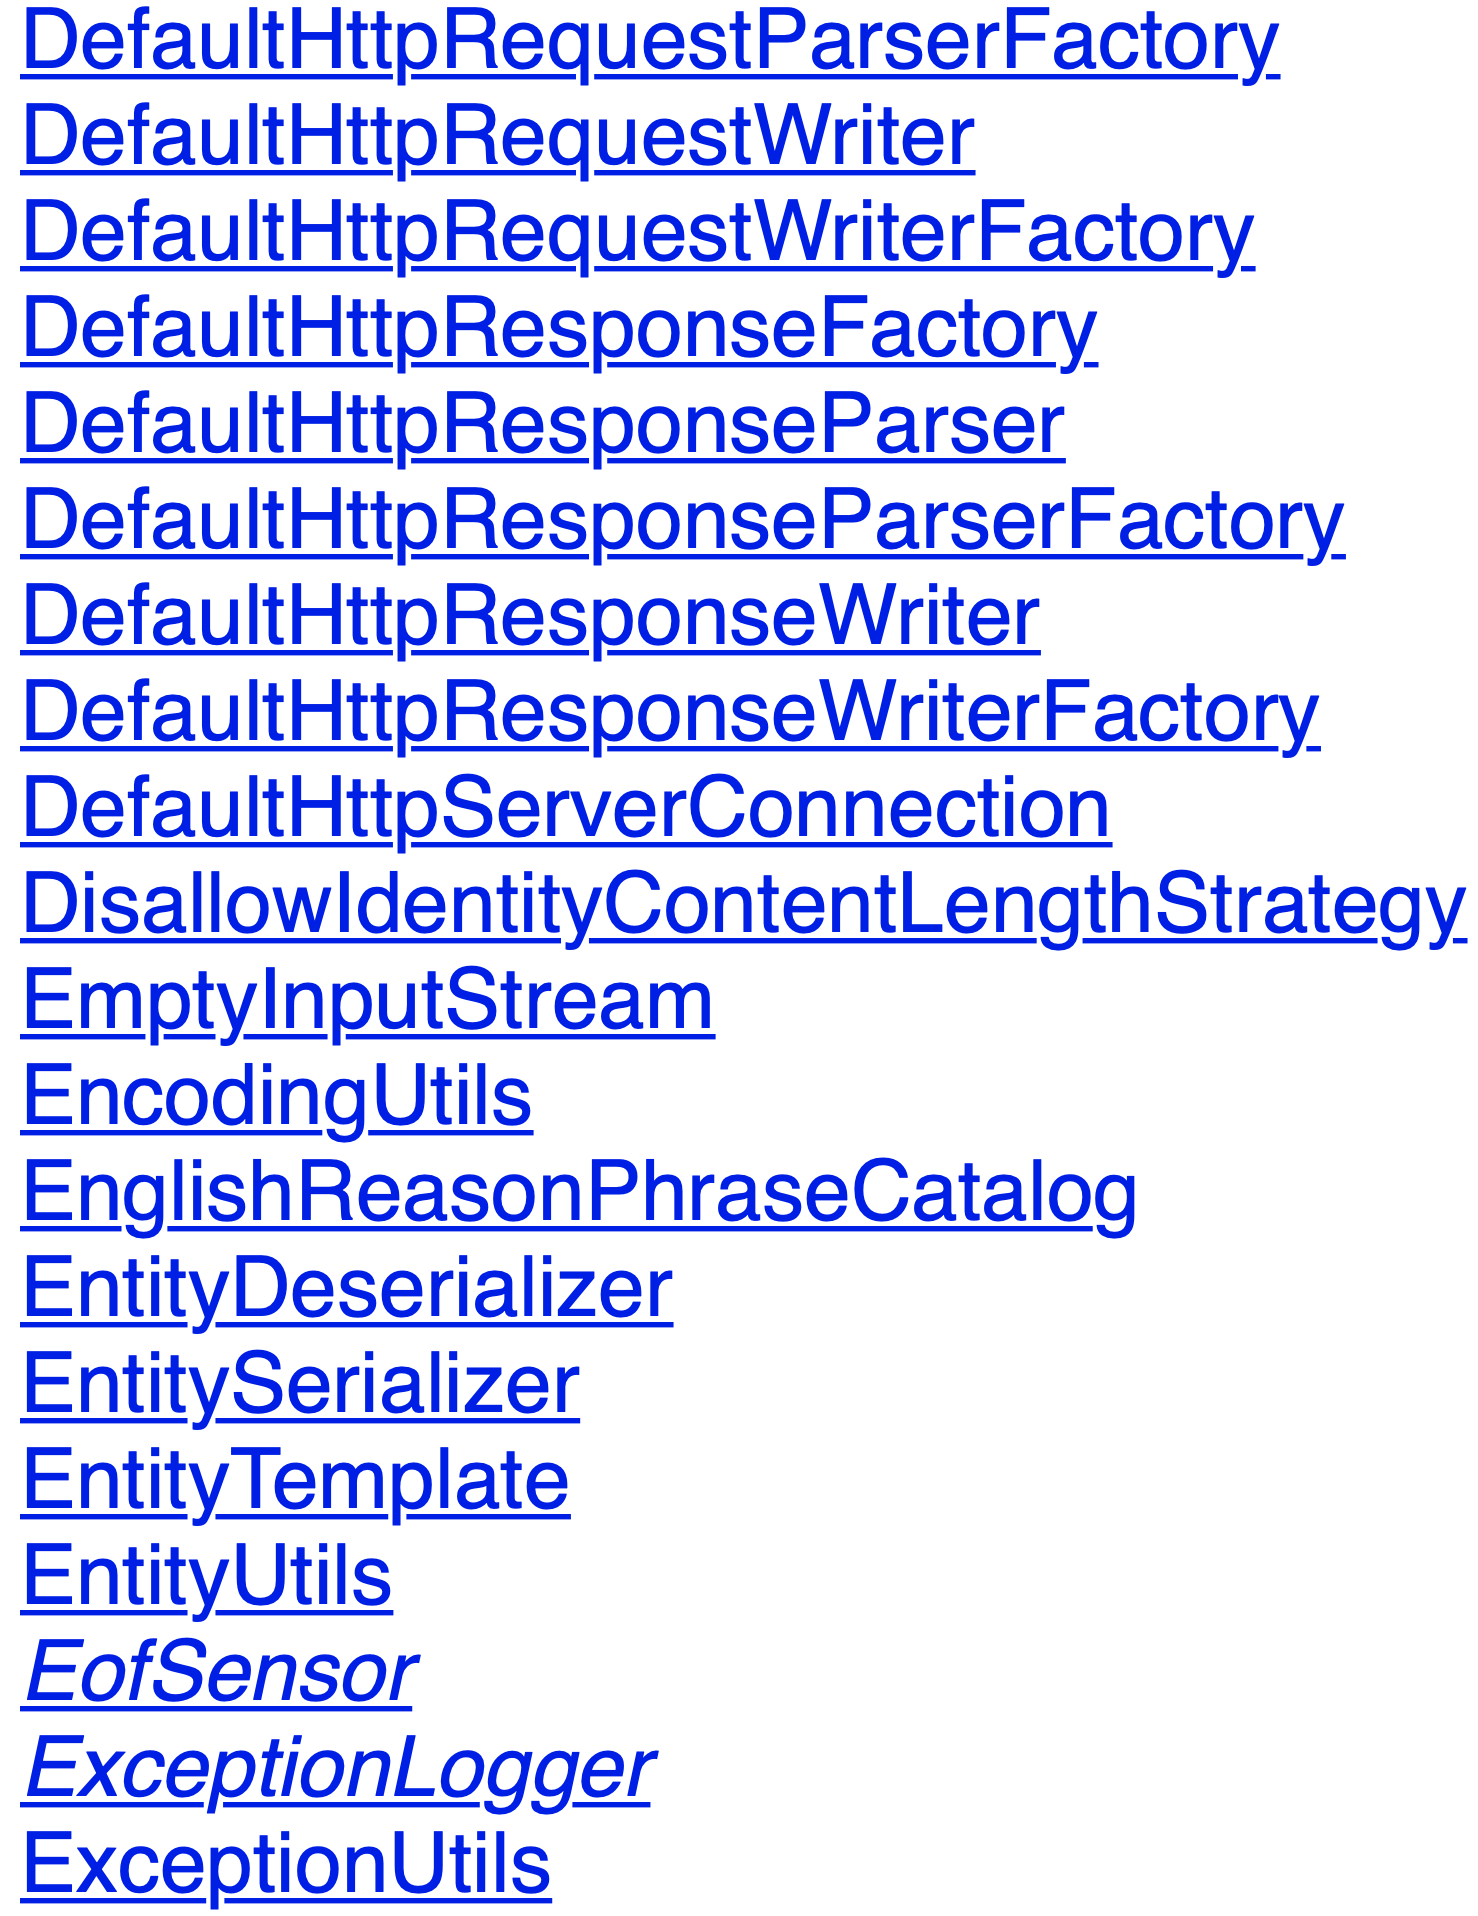
\includegraphics[width = 1in]{pics/15_all_classes.png}
				%\caption{fig1}
			\end{minipage}%
		}
		\subfigure[]{
			\begin{minipage}[t]{0.45\linewidth}
				\centering
				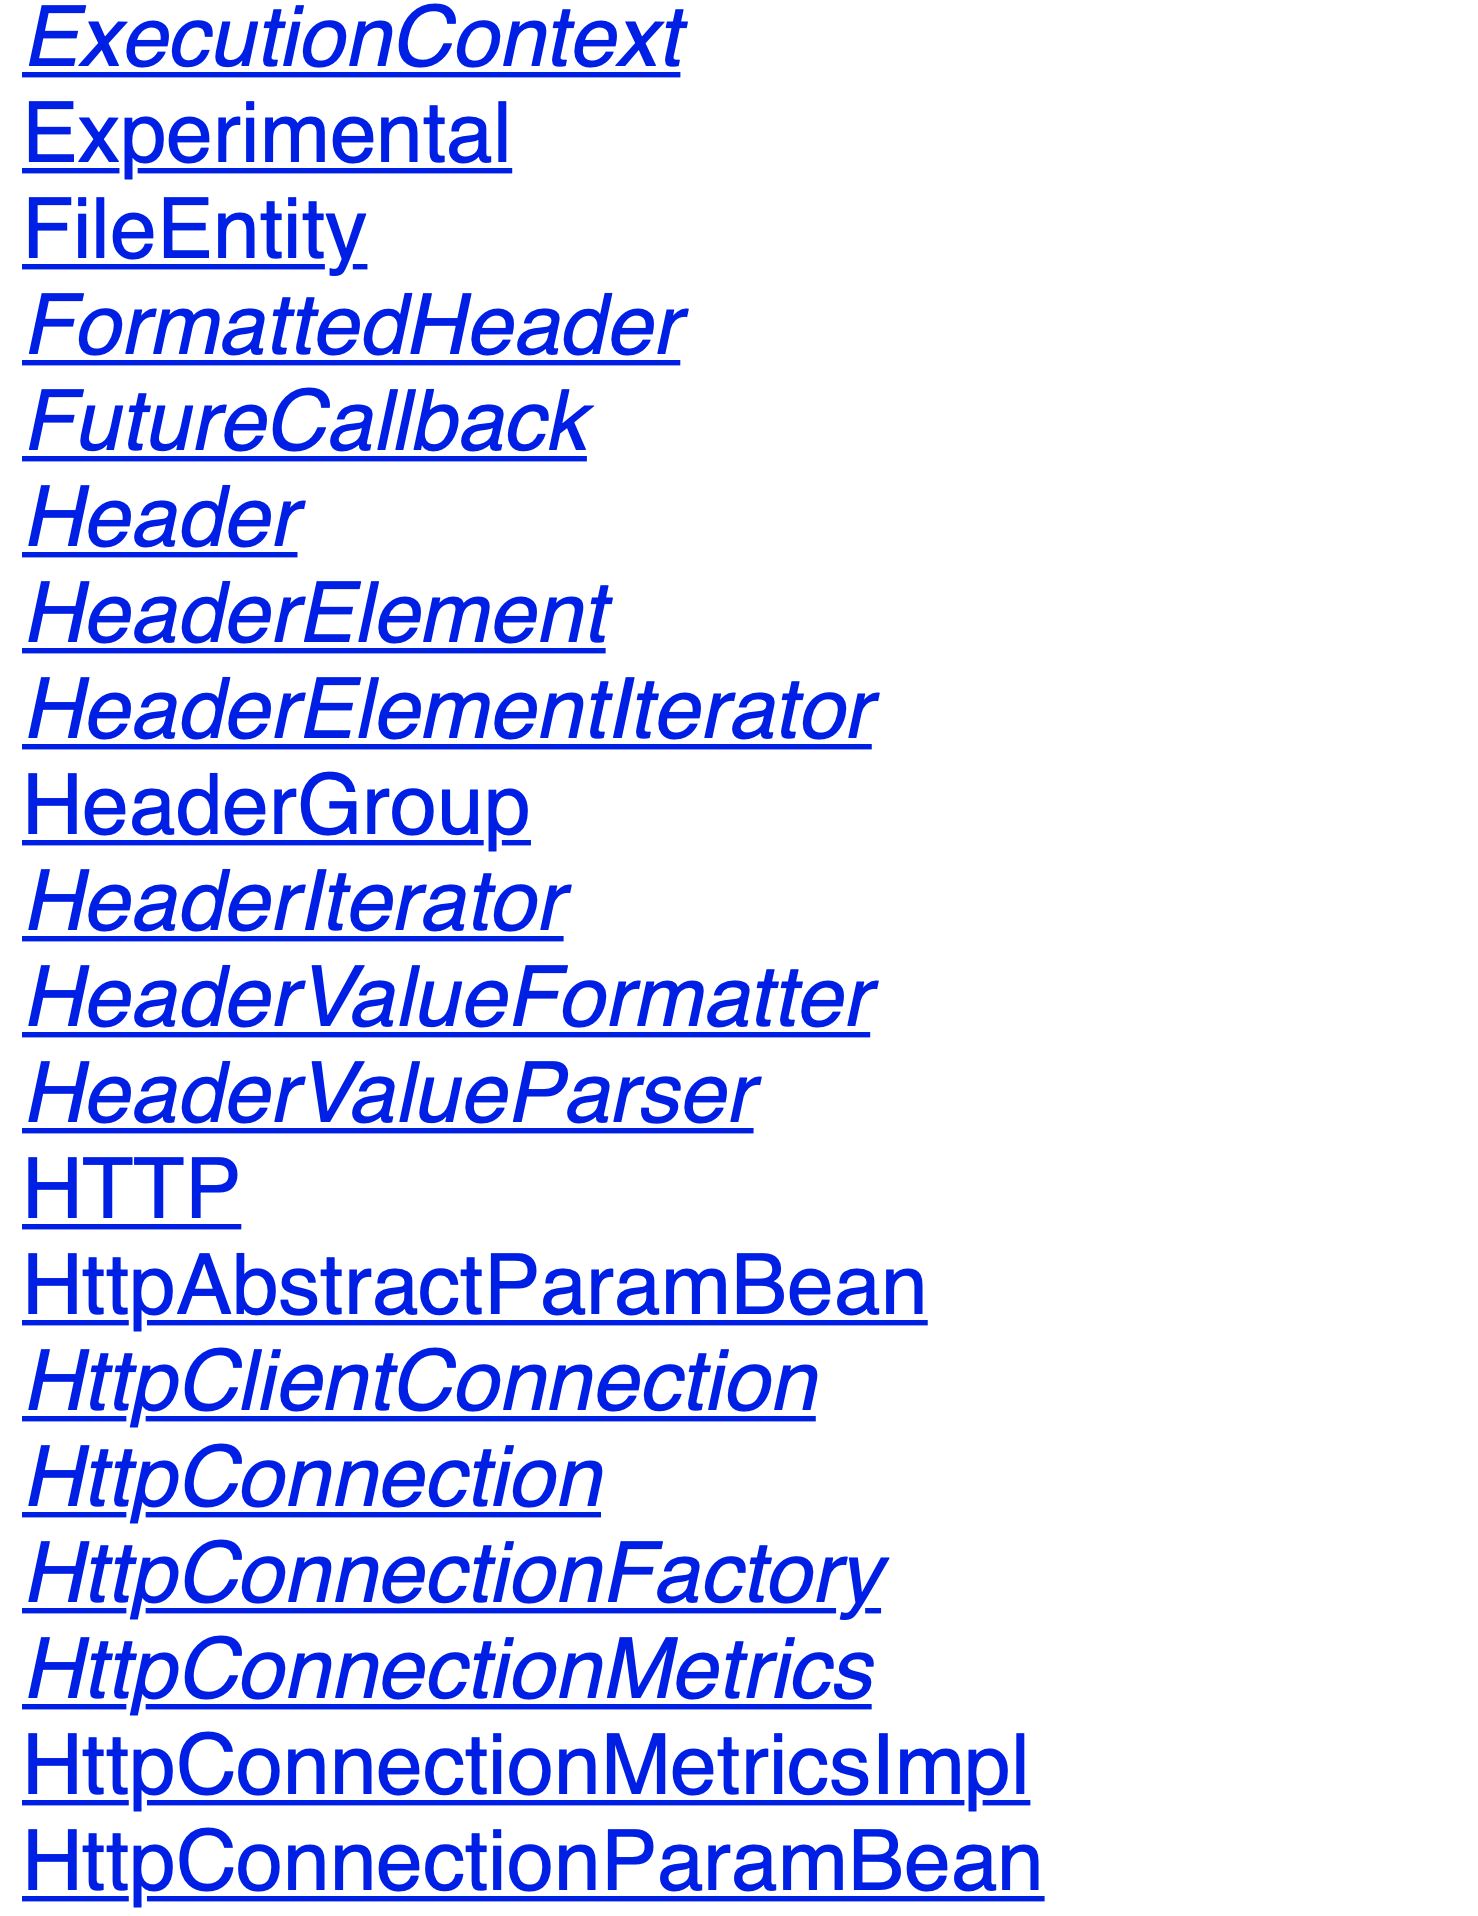
\includegraphics[width = 1in]{pics/16_all_classes.png}
				%\caption{fig2}
			\end{minipage}%
		}%
		\quad
		\subfigure[]{
			\begin{minipage}[t]{0.45\linewidth}
				\centering
				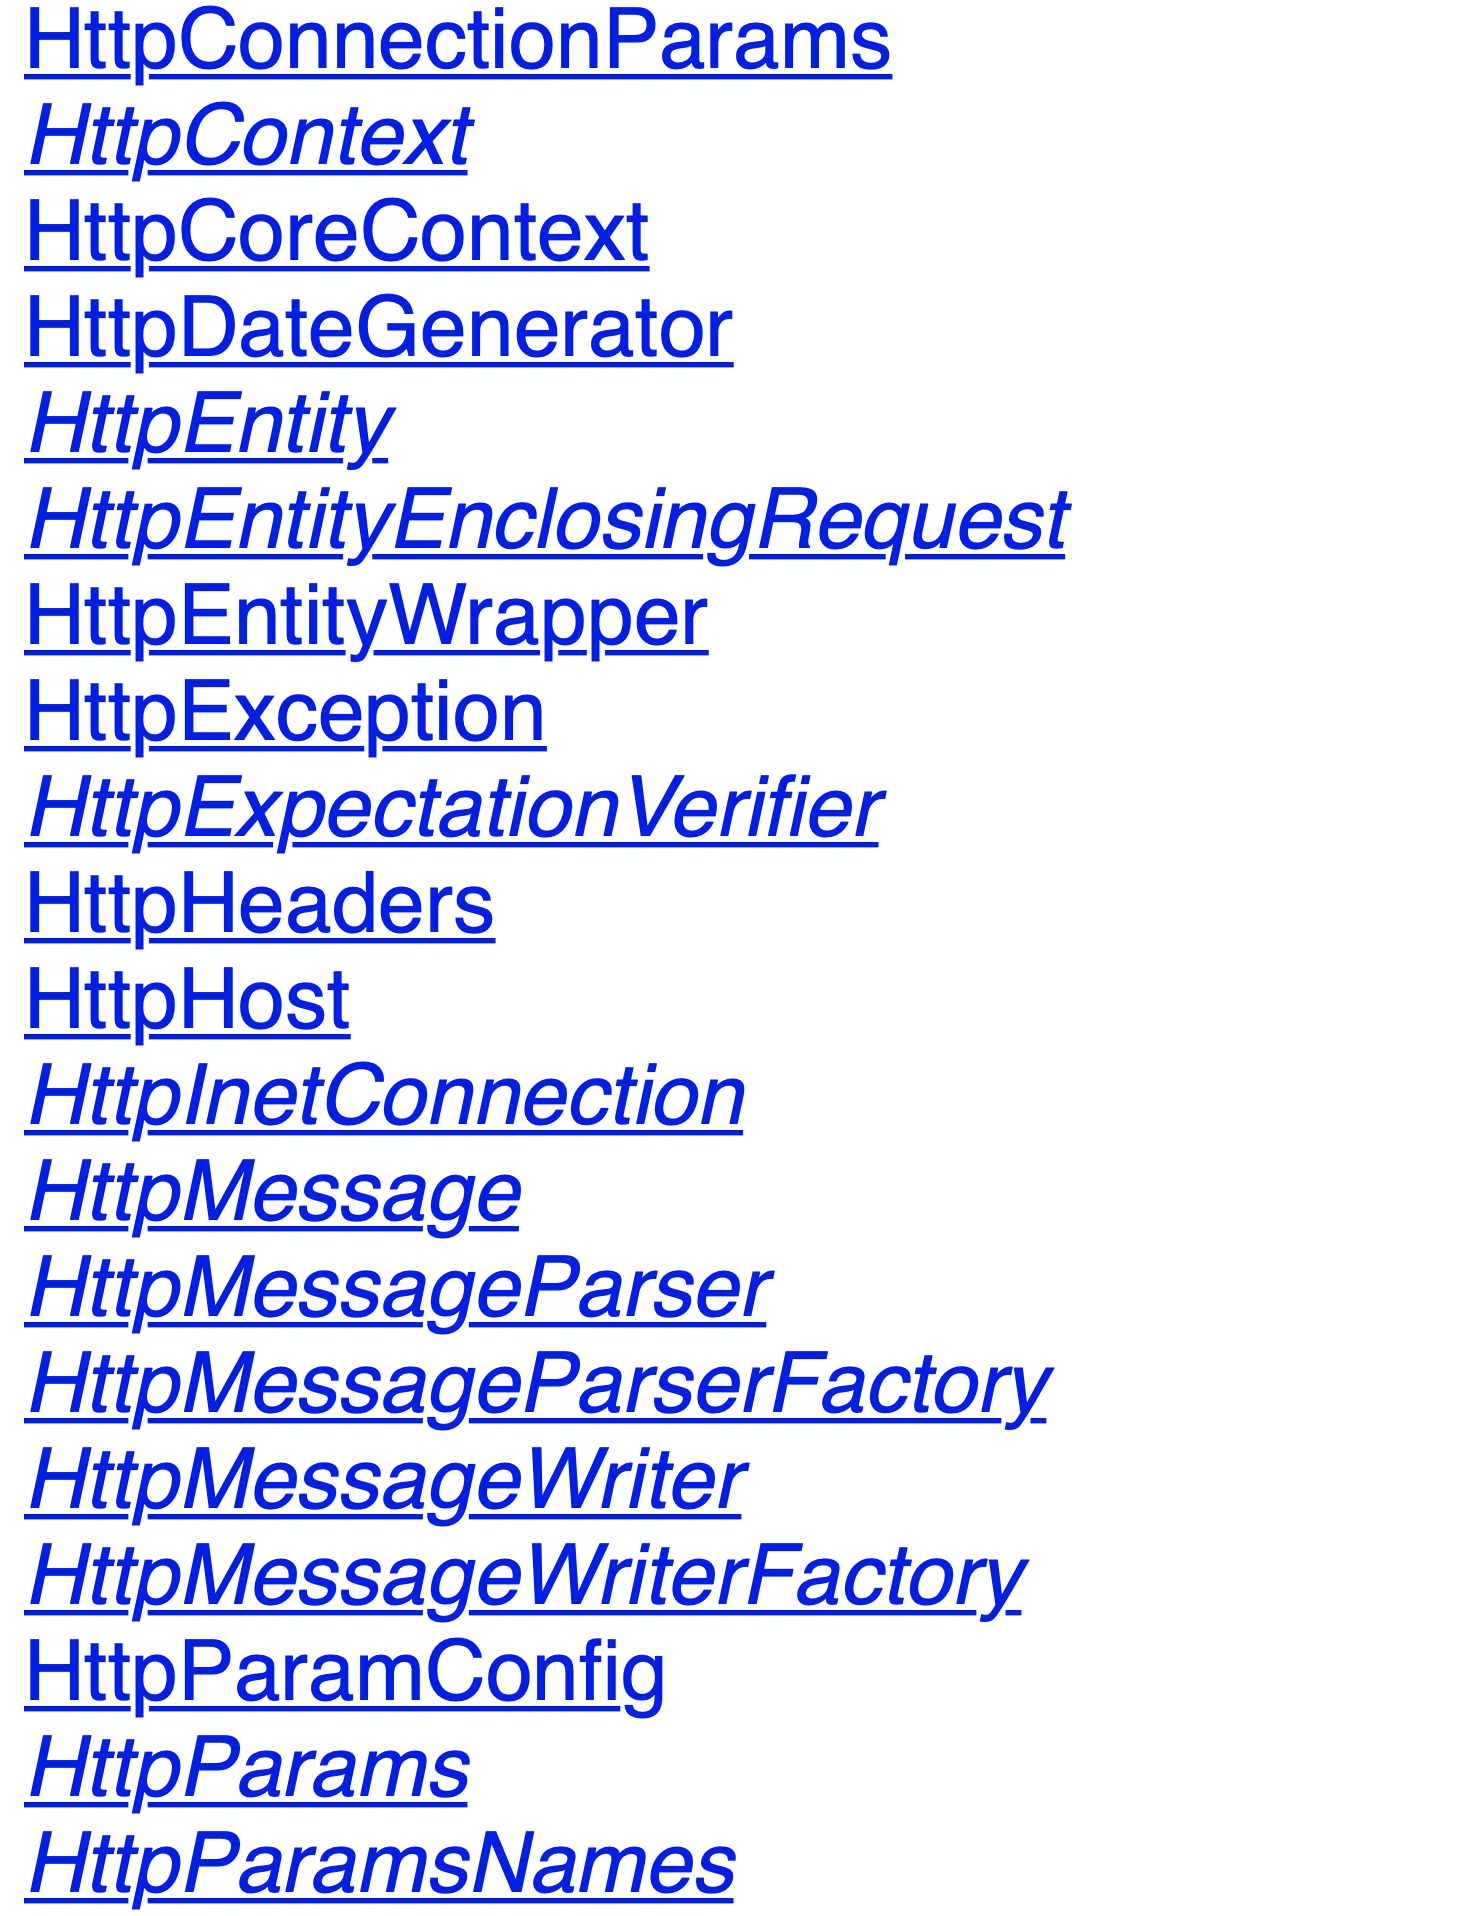
\includegraphics[width = 1in]{pics/17_all_classes.png}
				%\caption{fig2}
			\end{minipage}
		}%
		\subfigure[]{
			\begin{minipage}[t]{0.45\linewidth}
				\centering
				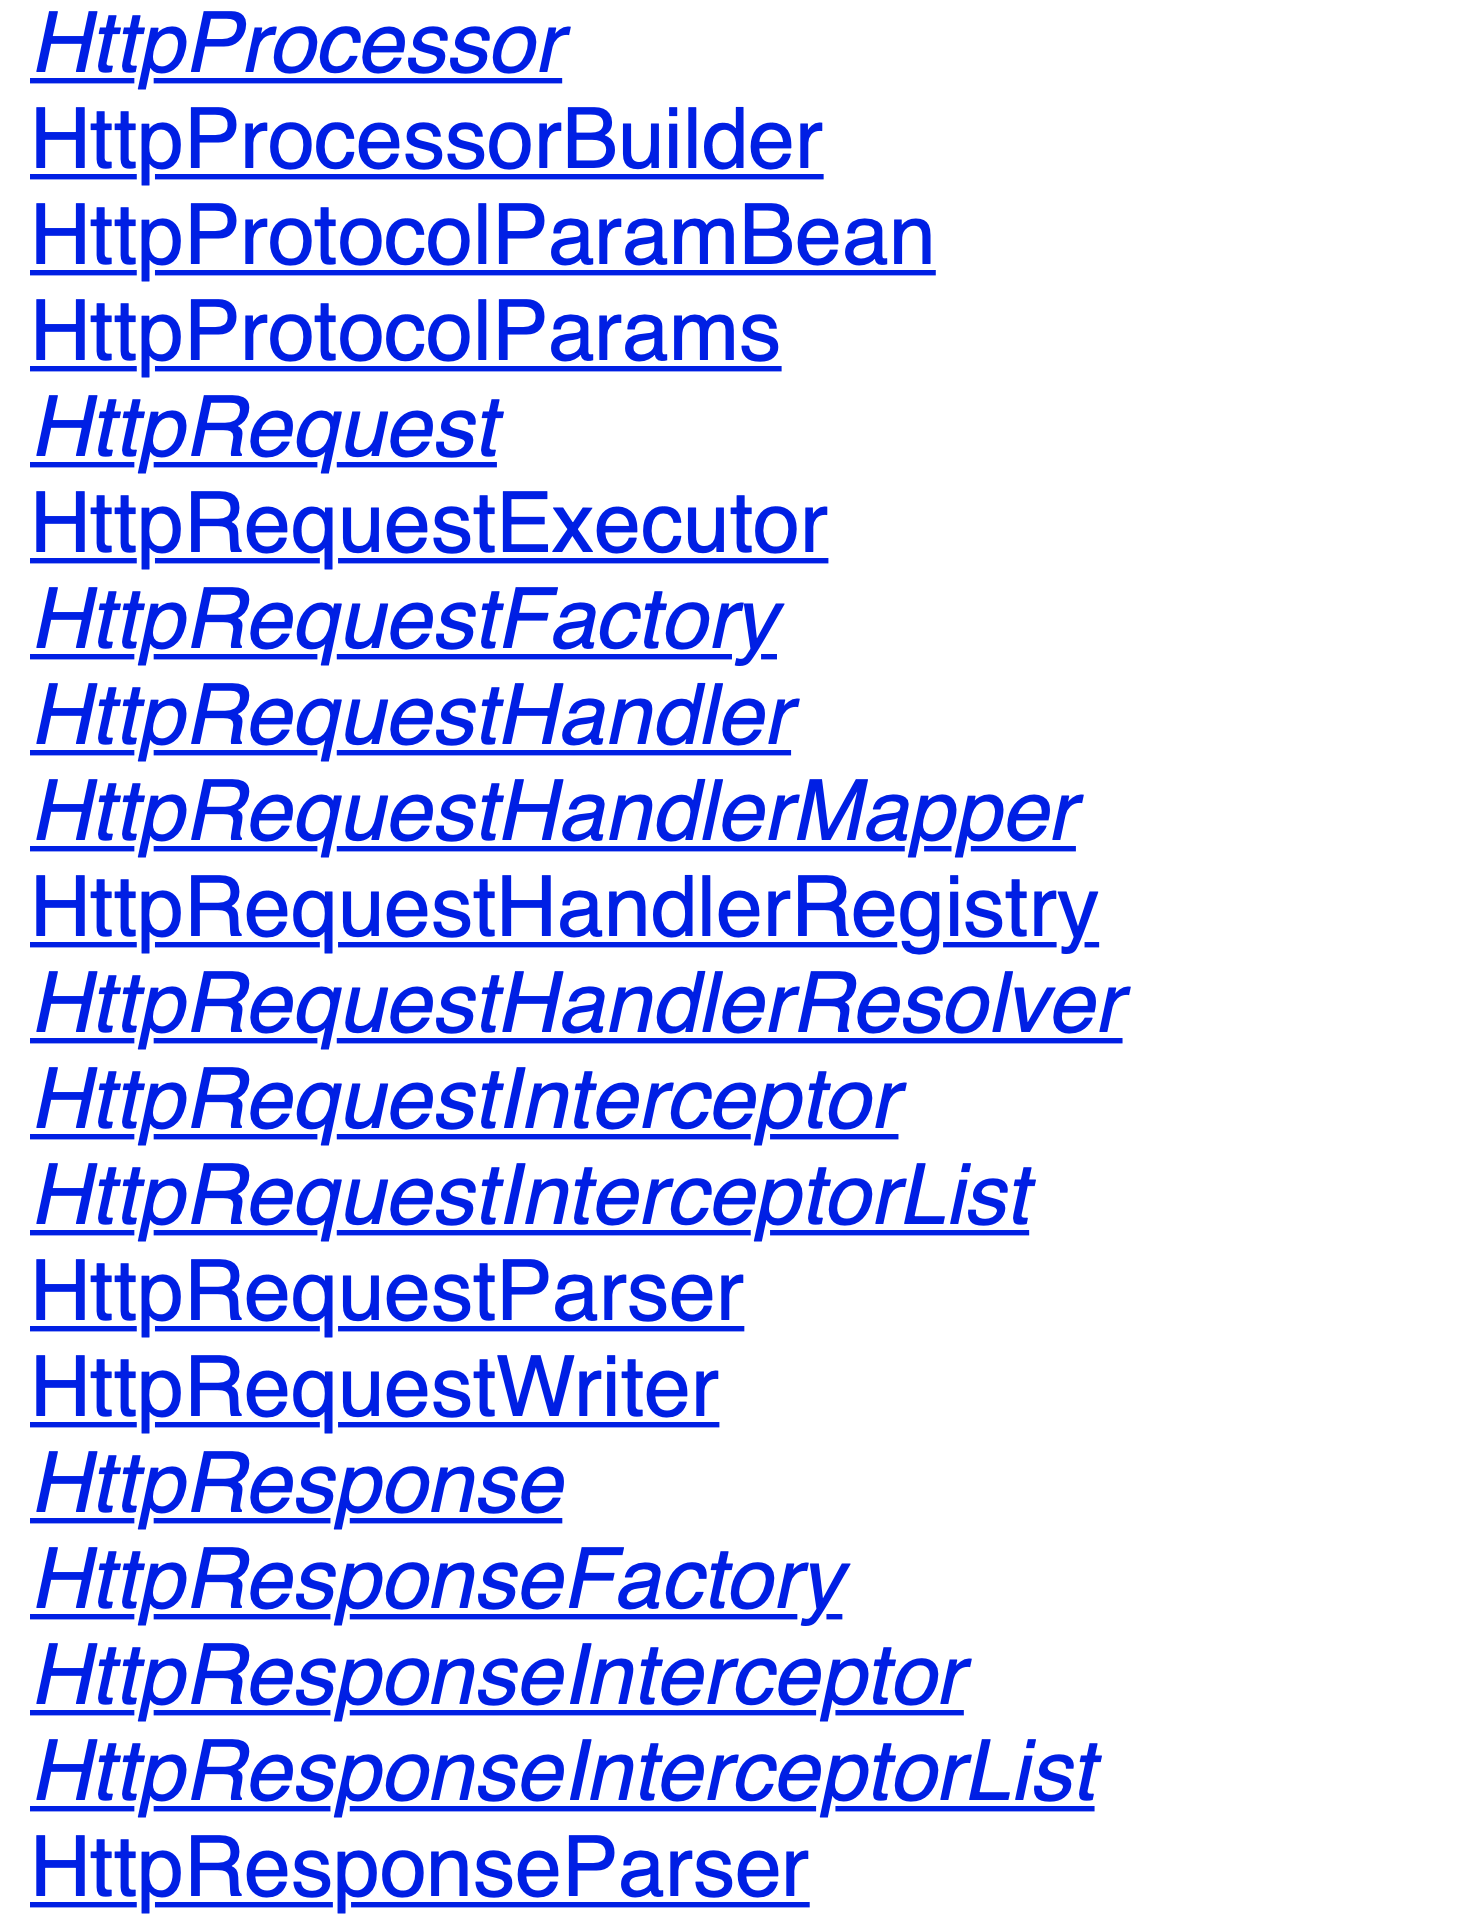
\includegraphics[width = 1in]{pics/18_all_classes.png}
				%\caption{fig2}
			\end{minipage}
		}%
		\quad
		\subfigure[]{
			\begin{minipage}[t]{0.45\linewidth}
				\centering
				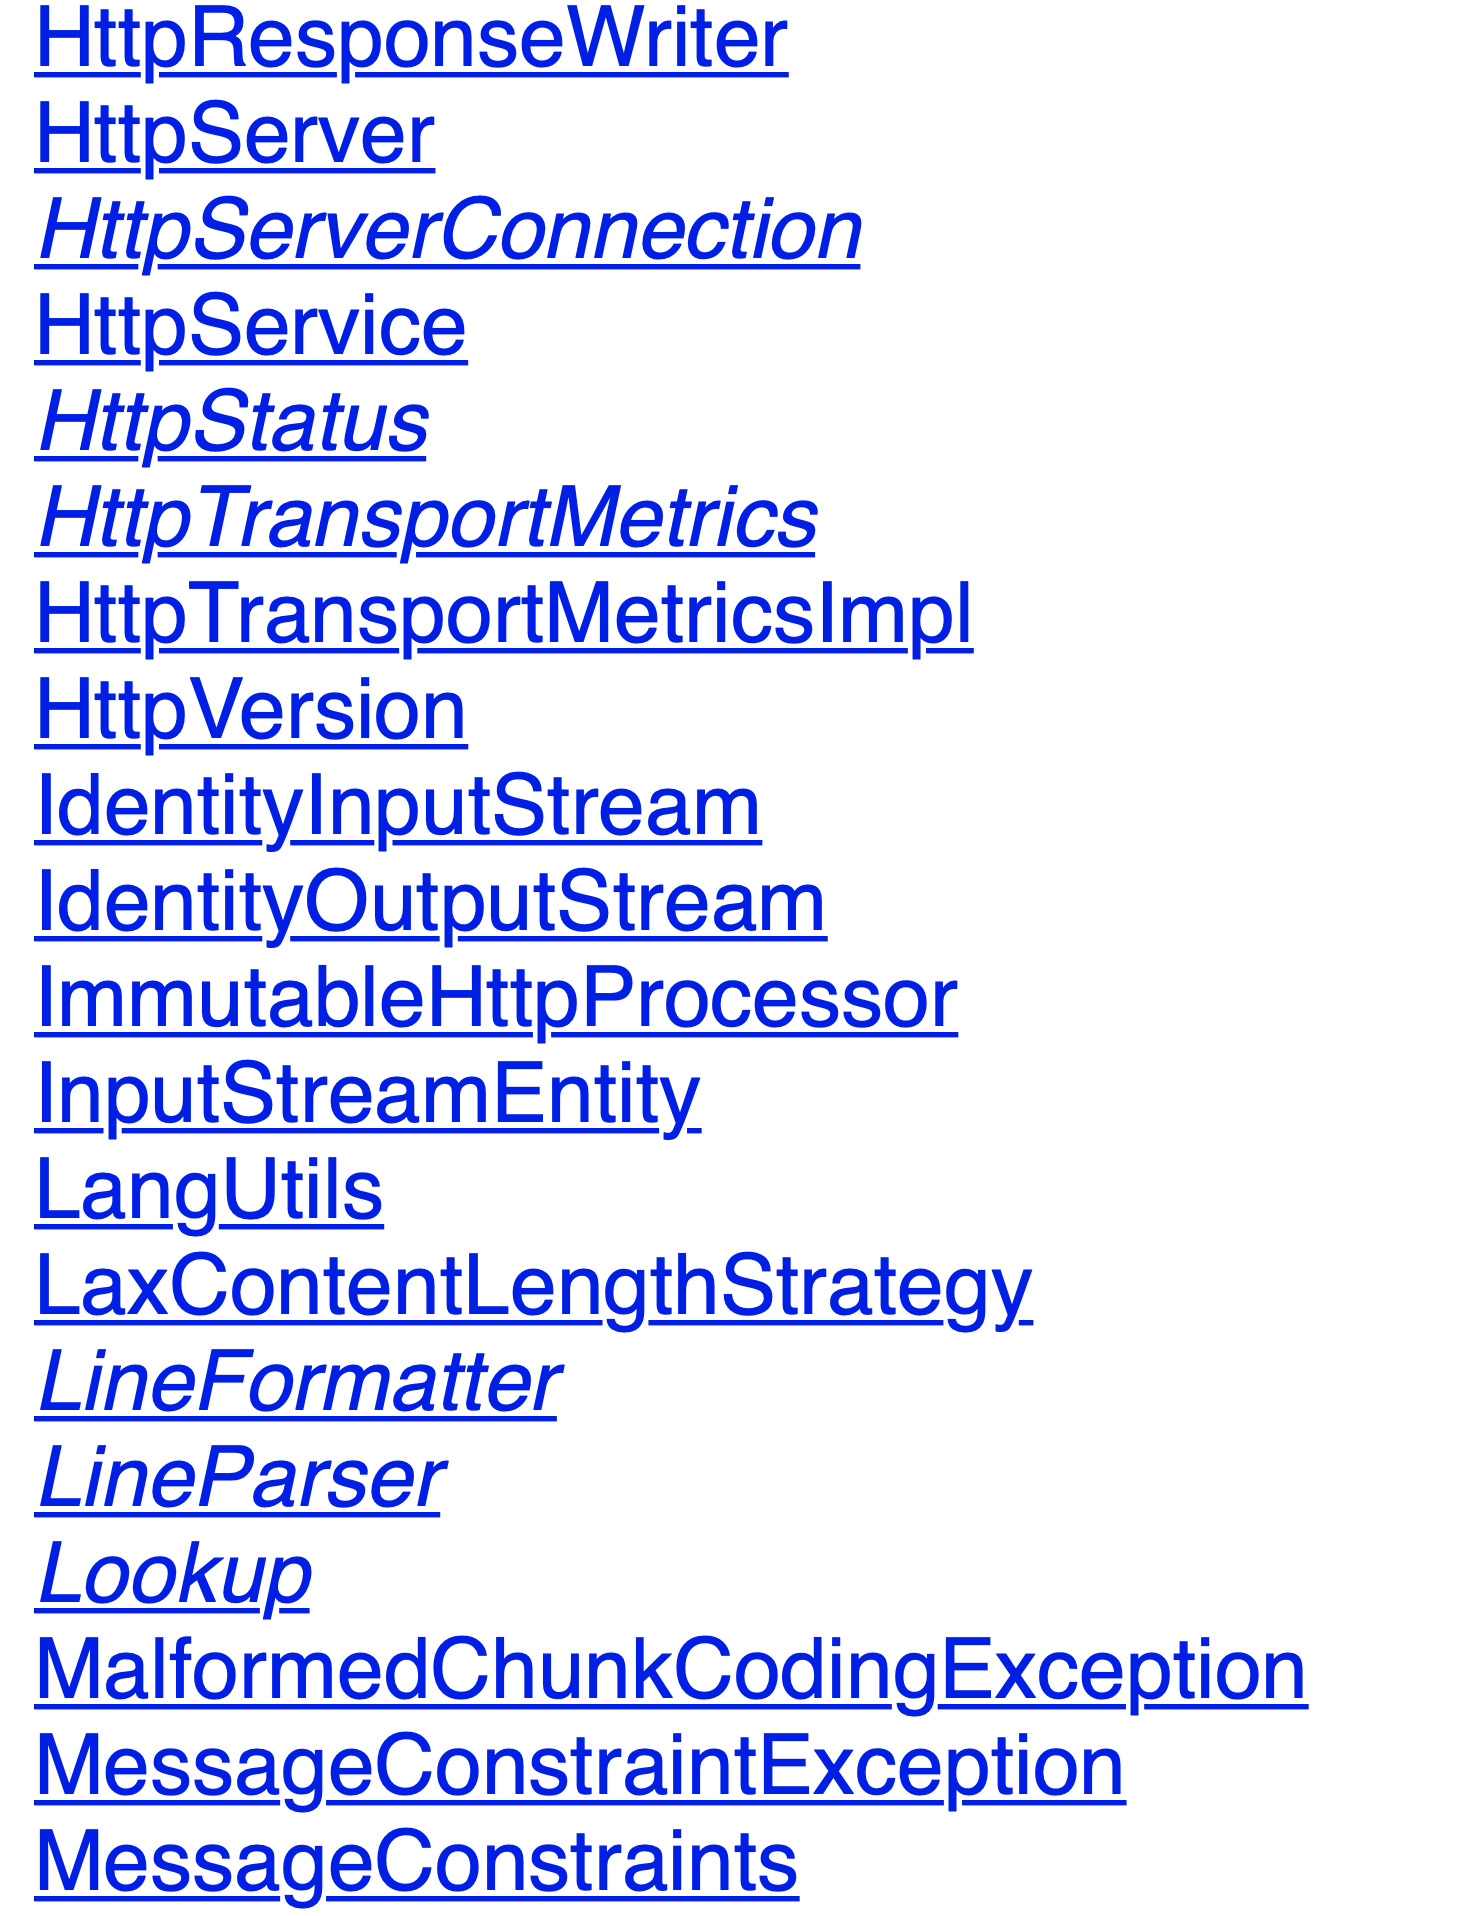
\includegraphics[width = 1in]{pics/19_all_classes.png}
				%\caption{fig2}
			\end{minipage}
		}%
		\subfigure[]{
			\begin{minipage}[t]{0.45\linewidth}
				\centering
				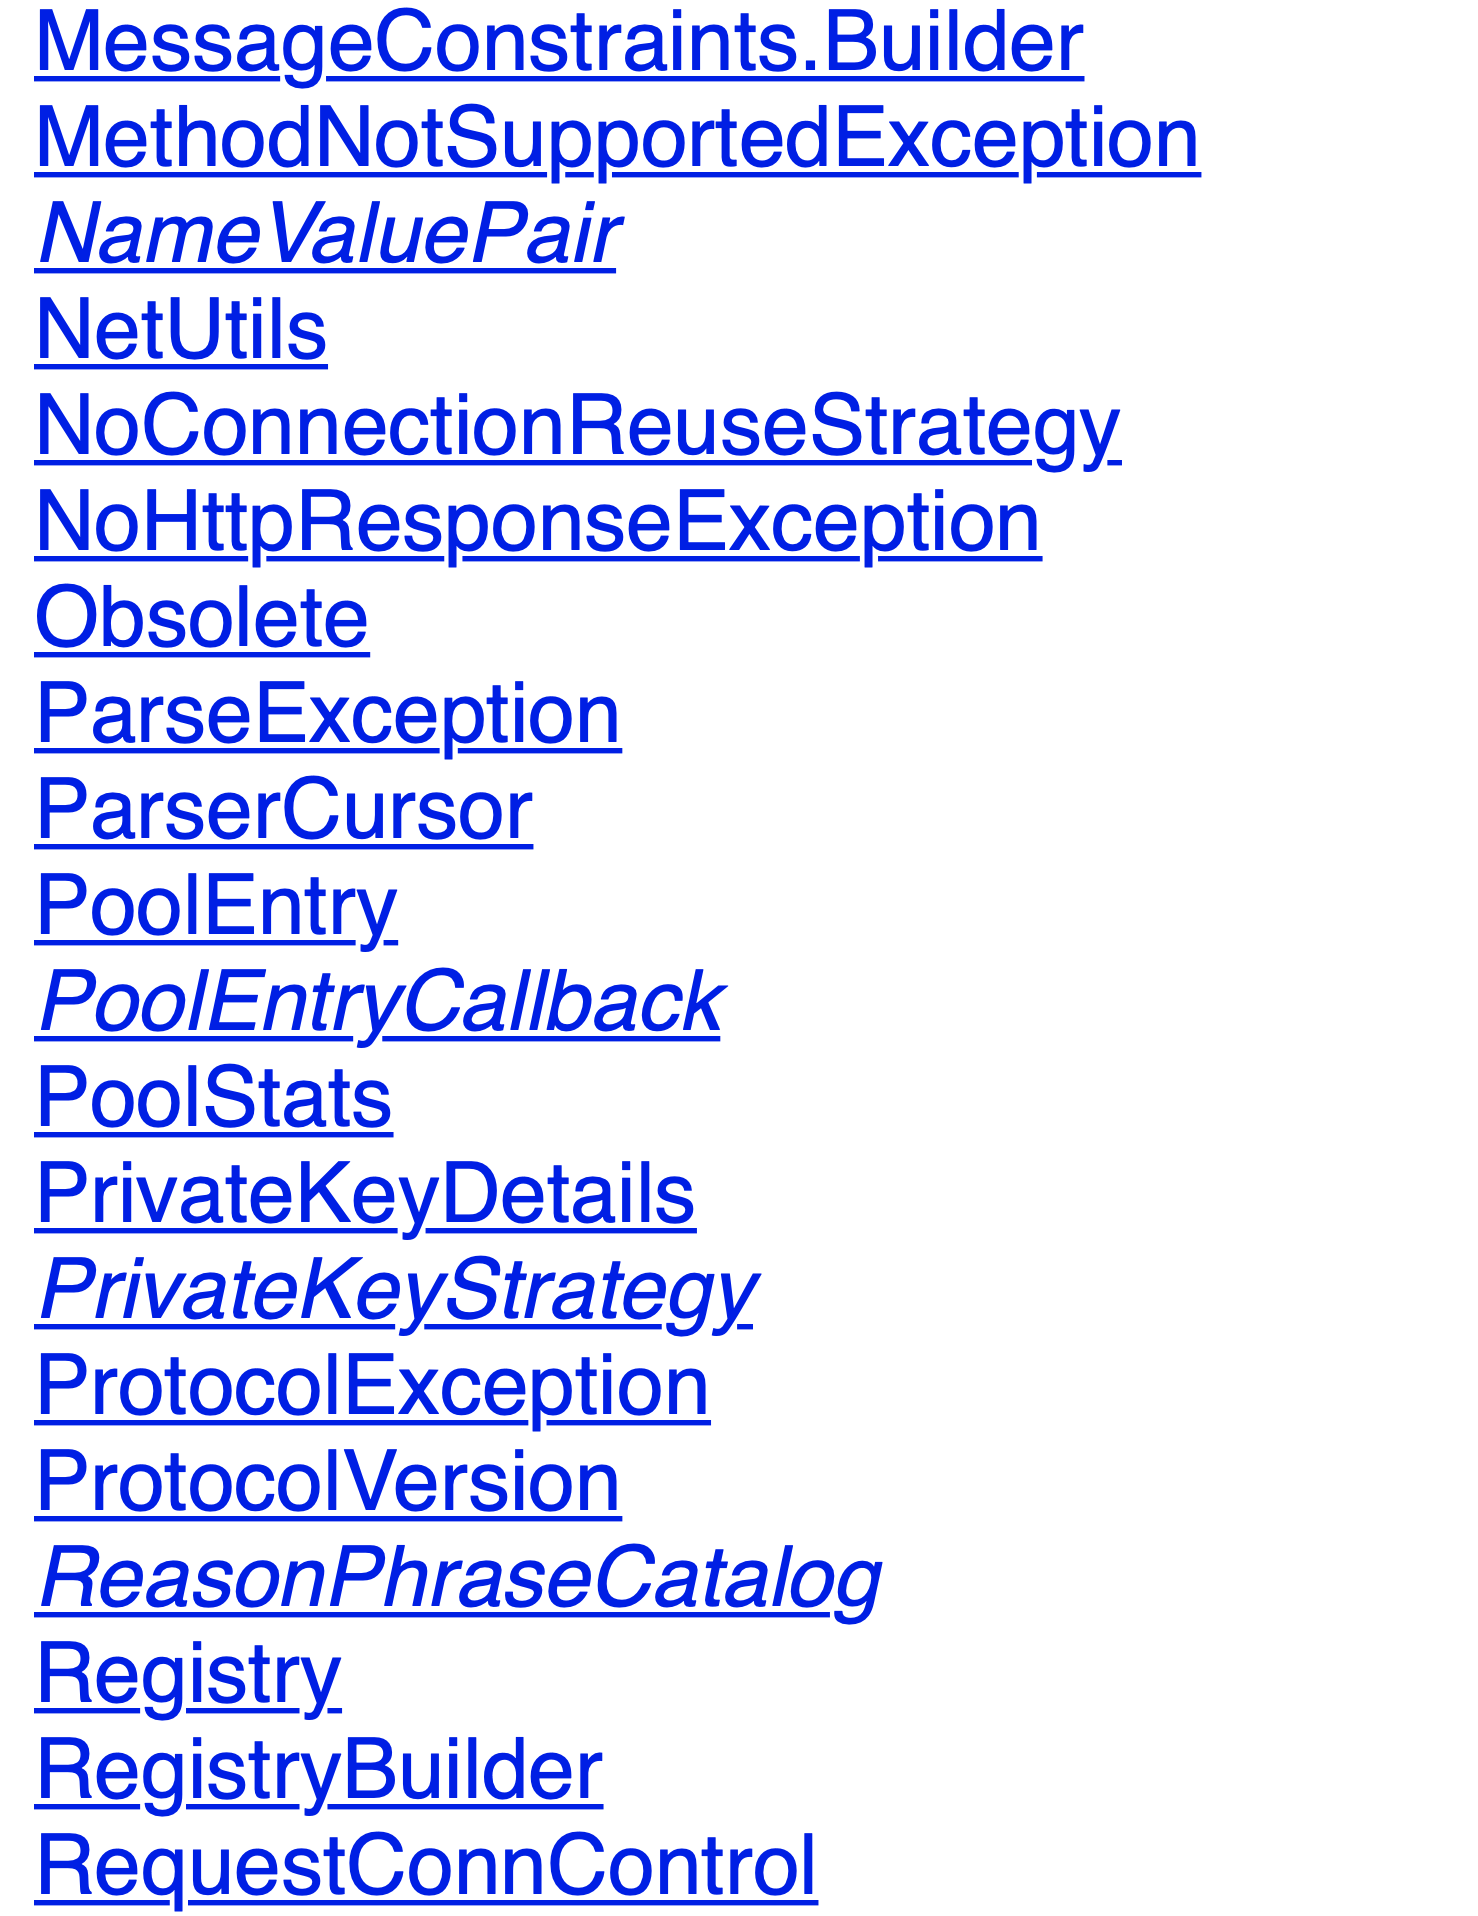
\includegraphics[width = 1in]{pics/20_all_classes.png}
				%\caption{fig2}
			\end{minipage}
		}%
		\quad
		\subfigure[]{
			\begin{minipage}[t]{0.45\linewidth}
				\centering
				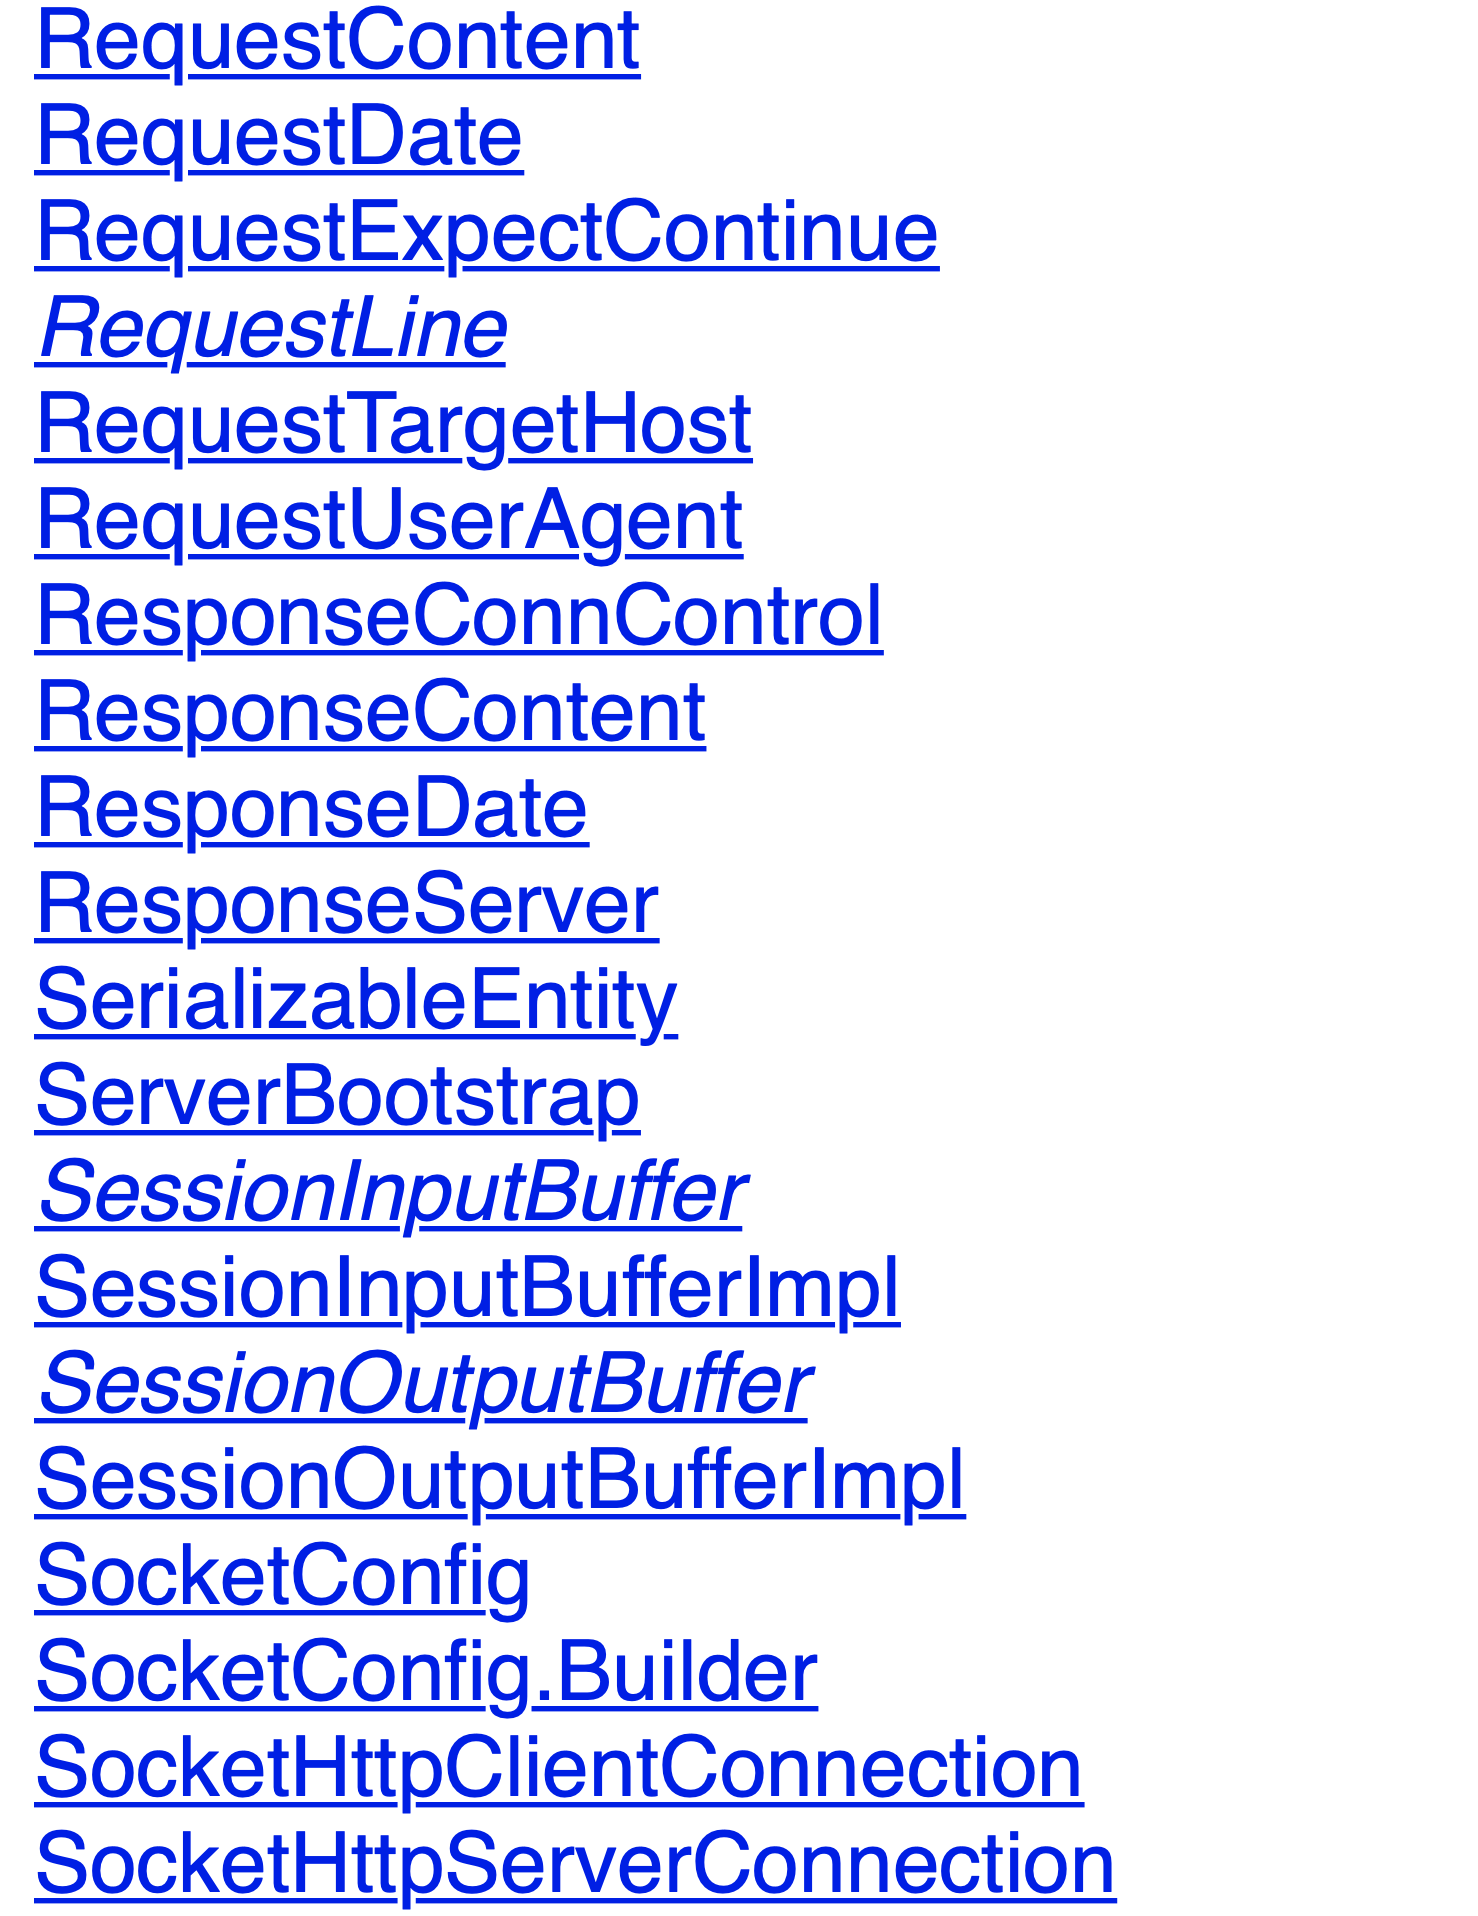
\includegraphics[width = 1in]{pics/21_all_classes.png}
				%\caption{fig2}
			\end{minipage}
		}%
		\subfigure[]{
			\begin{minipage}[t]{0.45\linewidth}
				\centering
				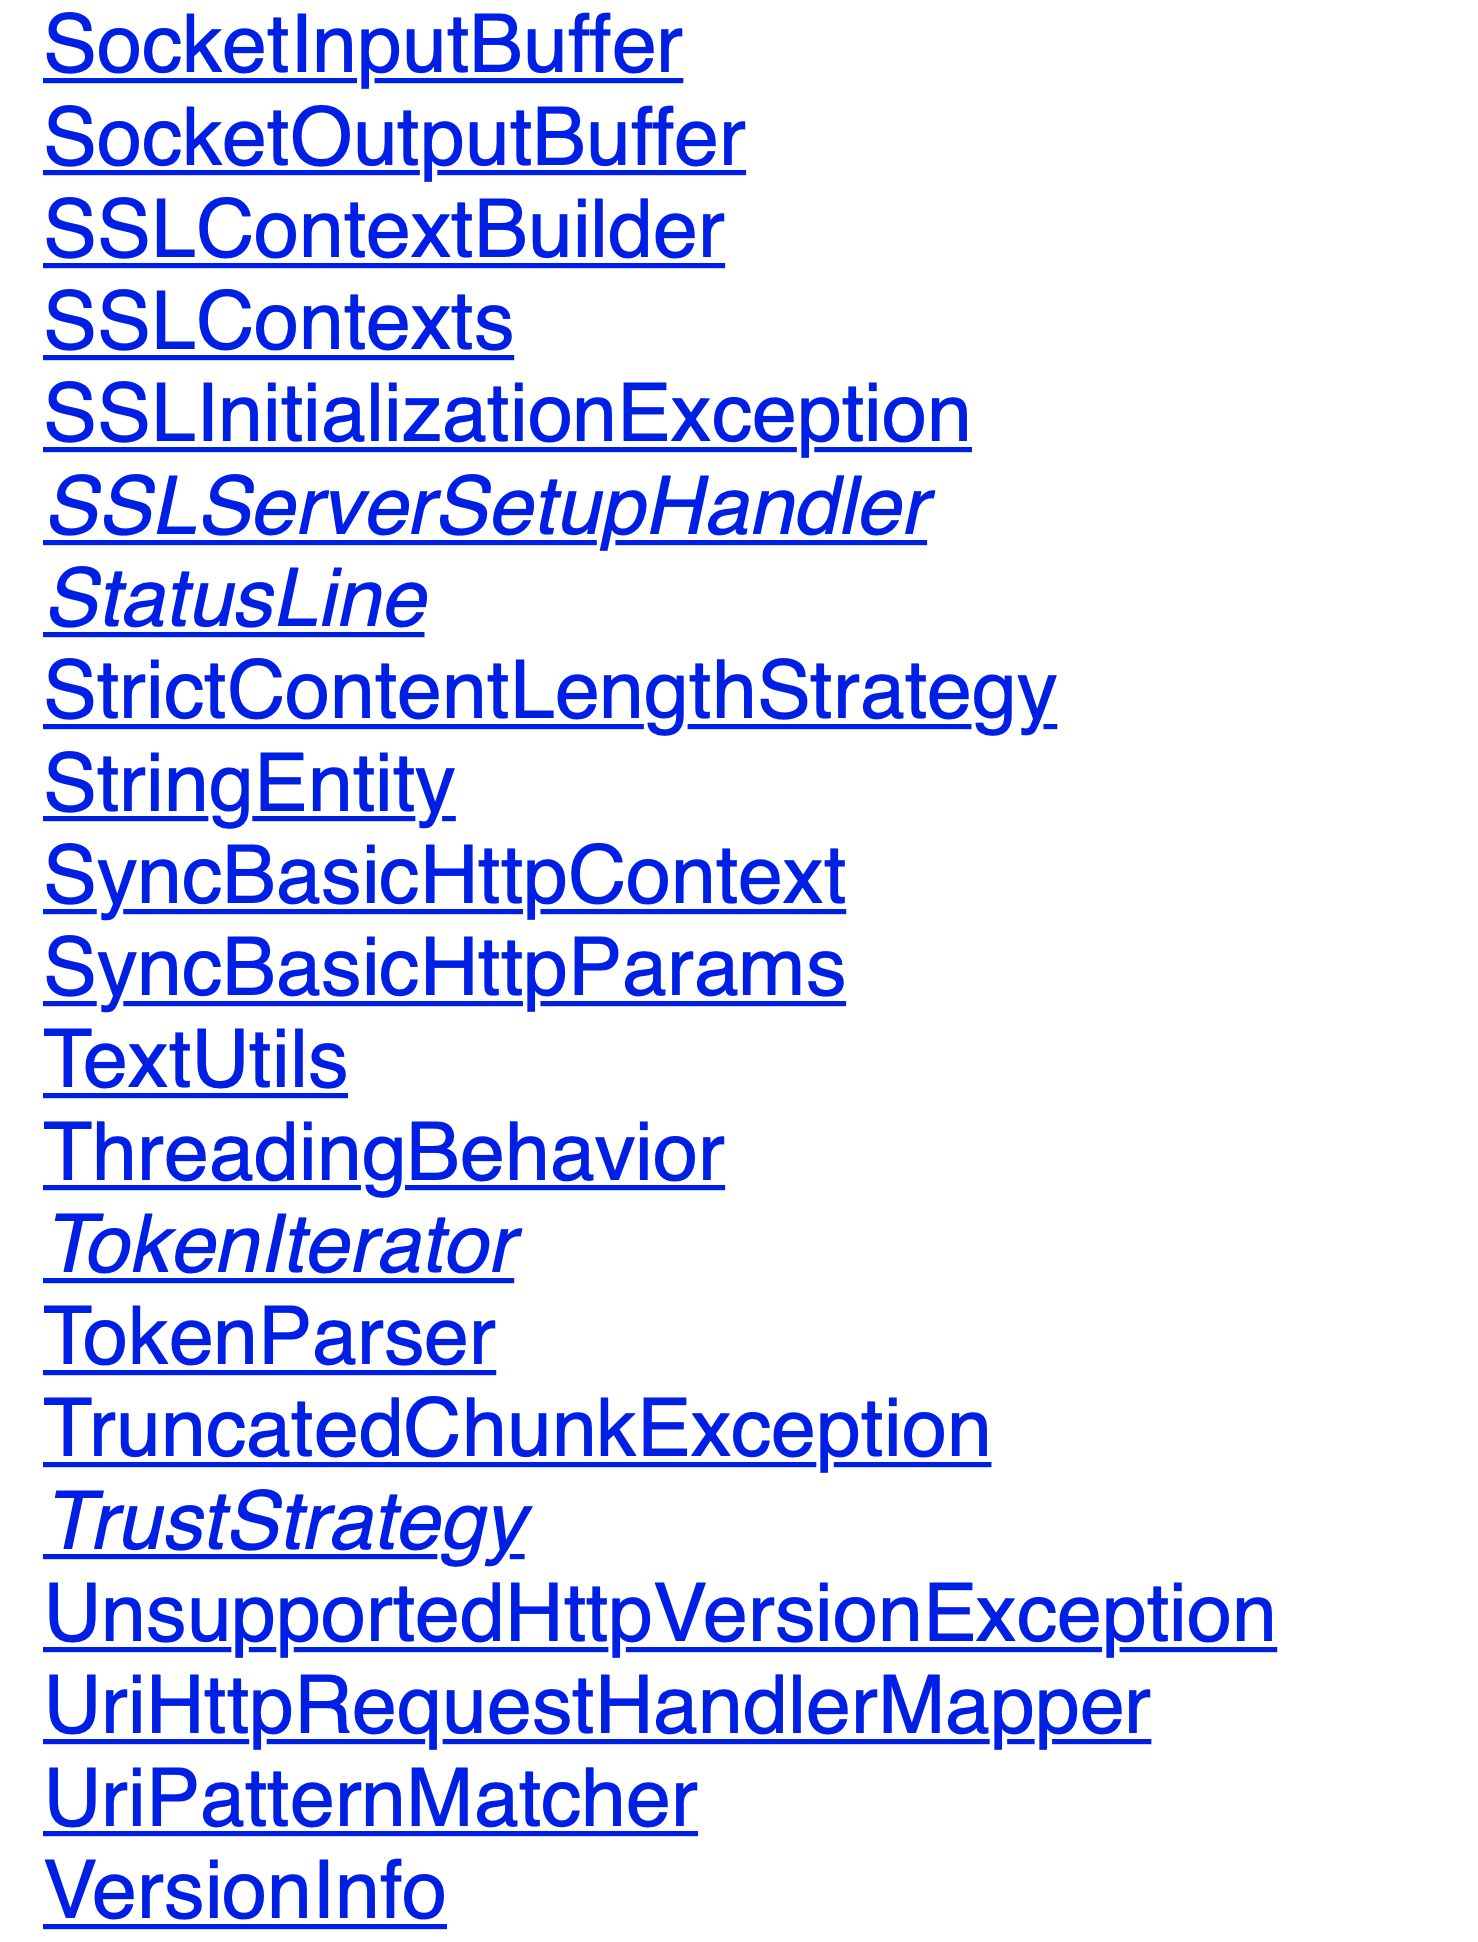
\includegraphics[width = 1in]{pics/22_all_classes.png}
				%\caption{fig2}
			\end{minipage}
		}%
		\centering
		\caption{Classes of HttpCore}
	\end{figure}

	\subsection{BasicHttpRequest}
	\begin{CJK}{UTF8}{gbsn}
		路径:org.apache.http.message\\
		继承: AbstractHttpMessage\\
		实现接口: HttpRequest
	\end{CJK}{}
	\subsubsection{Methods in BasicHttpRequest}
	\begin{CJK}{UTF8}{gbsn}
		\subparagraph{}
		BasicHttpRequest 中包含了从别的类中继承来的方法,以及其独有的,其关系如 Figure 9 所示。
	\end{CJK}{}
	\begin{figure}[H]
		\centering
		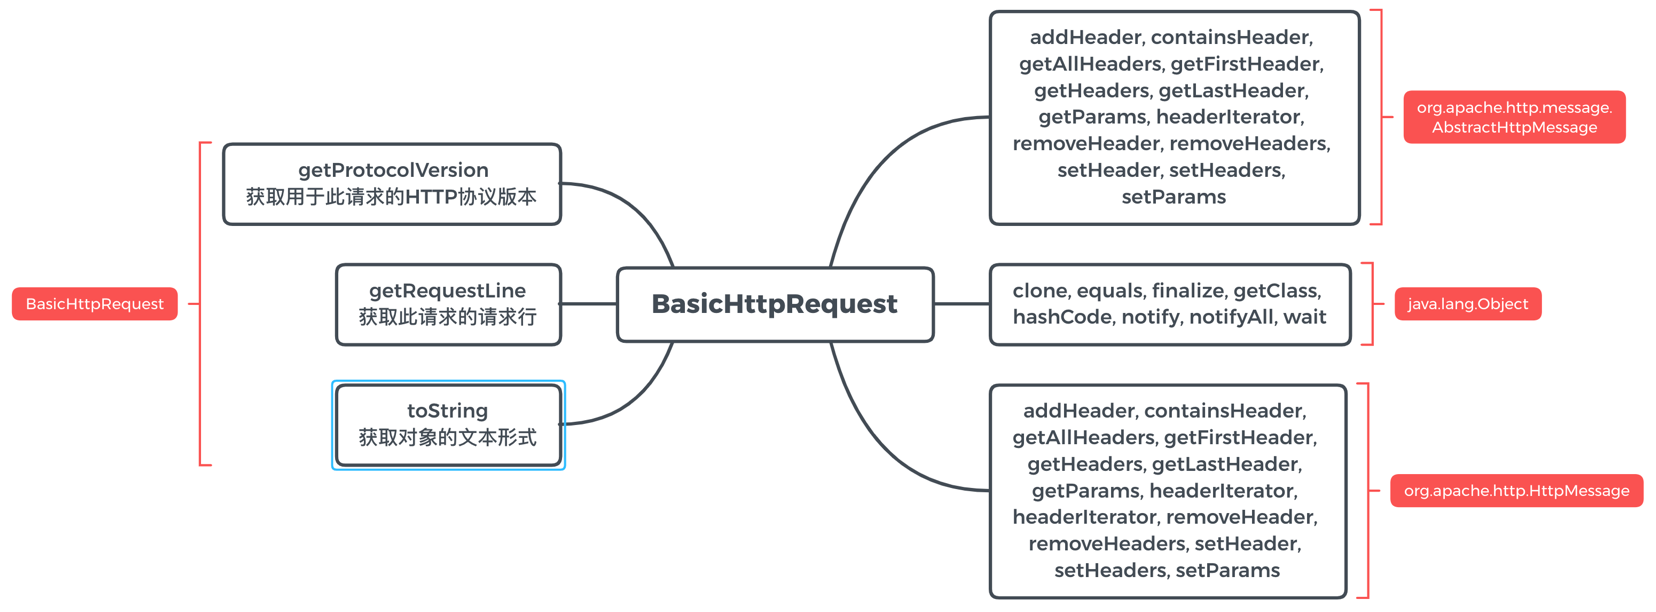
\includegraphics[height = 5cm, width = 15cm]{pics/15_BasicHttpRequest.png}	
		\caption{Methods in BasicHttpRequest}
	\end{figure}

	\subsubsection{Constructors}

	\begin{center}
	\fbox{
		\shortstack[l]{
	    	\begin{CJK}{UTF8}{gbsn}
				构造器:一个类里用于建立对象的方法,与类名相同,没有返回类型,不会被继承,且不会有范围修饰符。
			\end{CJK}{}\\
			\begin{CJK}{UTF8}{gbsn}
				Java允许构造器重载(一个类被允许拥有多个接受不同参数种类的构造器同时存在,方法名称相同,参数列表不同)
			\end{CJK}{}\\
			\begin{CJK}{UTF8}{gbsn}
				如果一个类中没有构造方法,那么编译器会为类加上一个默认的构造方法。
构造器在创建对象的时候调用,为
			\end{CJK}{}\\
			\begin{CJK}{UTF8}{gbsn}
				正在创建的对象的成员变量赋初值。
			\end{CJK}{}
		}
	}
	\end{center}

	\begin{CJK}{UTF8}{gbsn}
		一个默认的构造方法的例子:
	\end{CJK}{}

	\begin{lstlisting}[language={java}]
/* Default Constructor */
public ClassName() {
	
}
	\end{lstlisting}

	\begin{figure}[H]
		\centering
		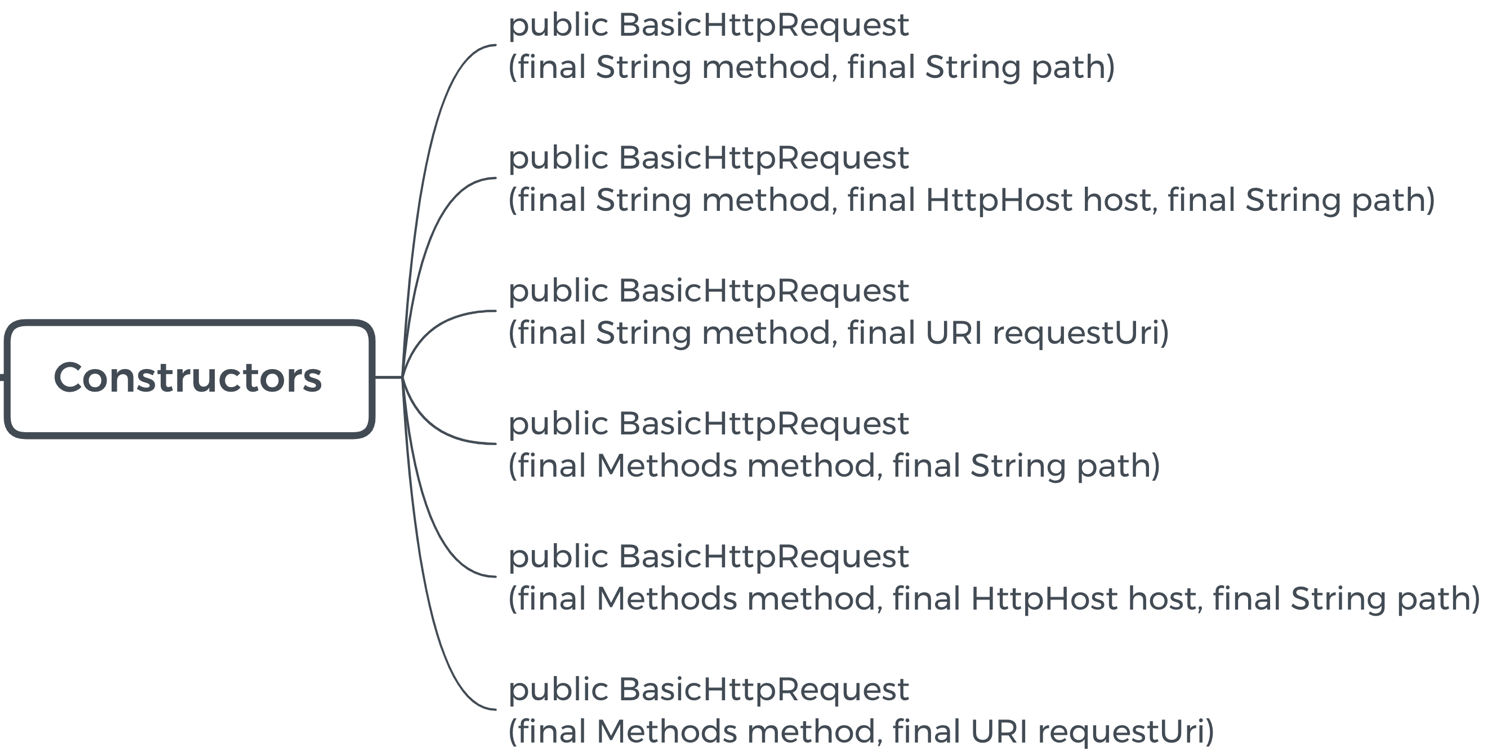
\includegraphics[height = 8cm, width = 13cm]{pics/17_Request_constructors.png}	
		\caption{Constructors in BasicHttpRequest}
	\end{figure}
	\begin{CJK}{UTF8}{gbsn}
		接下来分别介绍 BasicHttpRequest 中的构造器
	\end{CJK}{}
	\clearpage
	%\renewcommand{\baselinestretch}{1.0}
	\begin{lstlisting}[language={java}]
/**
 * Creates request message with the given method and request path.
 *
 * @param method request method.
 * @param path request path.
 */
public BasicHttpRequest(final String method, final String path) {
    super();
    this.method = method;
    if (path != null) {
        try {
            setUri(new URI(path));
        } catch (final URISyntaxException ex) {
            this.path = path;
        }
    }
}

	\end{lstlisting}
	\begin{figure}[H]
		\centering
		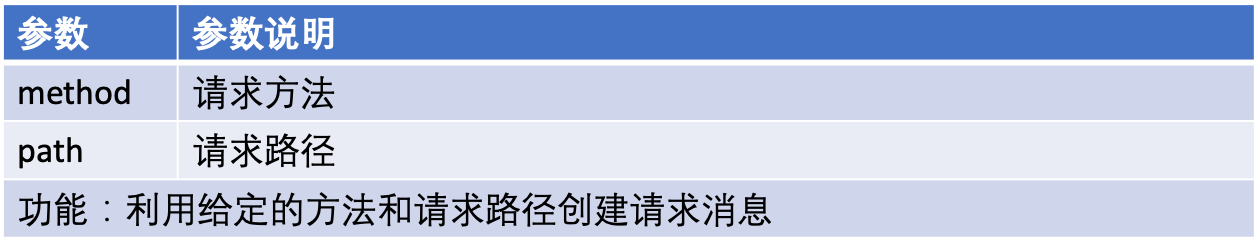
\includegraphics[height = 3.5cm, width = 18cm]{pics/18_Request_table_1_4.png}	
		%\caption{Constructors in BasicHttpRequest}
	\end{figure}

	\begin{lstlisting}[language={java}]
/**
 * Creates request message with the given method, host and request path.
 *
 * @param method request method.
 * @param host request host.
 * @param path request path.
 *
 * @since 5.0
 */
public BasicHttpRequest(final String method, final HttpHost host, final String path) {
    super();
    this.method = Args.notNull(method, "Method name");
    this.scheme = host != null ? host.getSchemeName() : null;
    this.authority = host != null ? new URIAuthority(host) : null;
    this.path = path;
}

	\end{lstlisting}
	\begin{figure}[H]
		\centering
		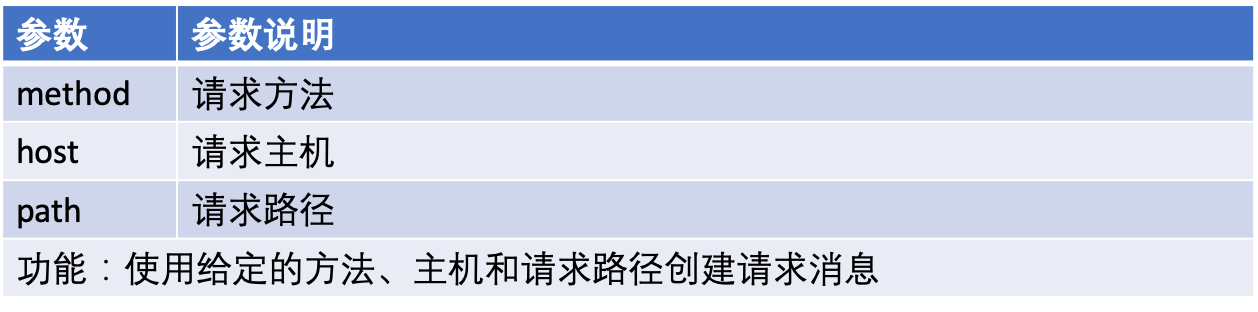
\includegraphics[height = 3.5cm, width = 18cm]{pics/19_Request_table_2_5.png}	
		%\caption{Constructors in BasicHttpRequest}
	\end{figure}

	\begin{lstlisting}[language={java}]
/**
 * Creates request message with the given method, request URI.
 *
 * @param method request method.
 * @param requestUri request URI.
 *
 * @since 5.0
 */
public BasicHttpRequest(final String method, final URI requestUri) {
    super();
    this.method = Args.notNull(method, "Method name");
    setUri(Args.notNull(requestUri, "Request URI"));
}

	\end{lstlisting}
	\begin{figure}[H]
		\centering
		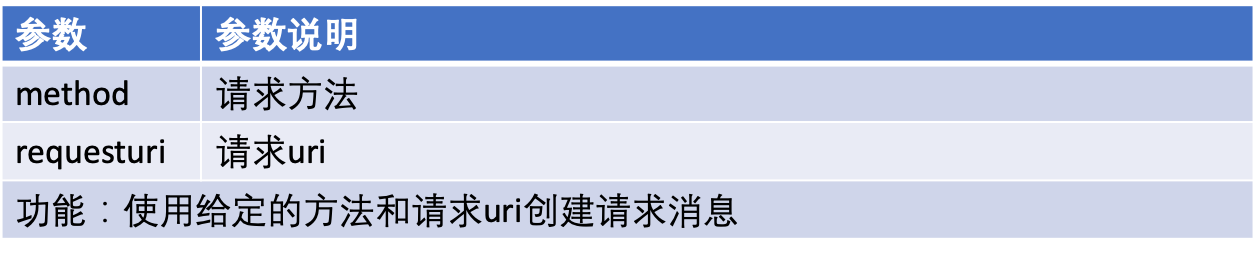
\includegraphics[height = 3.5cm, width = 18cm]{pics/20_Request_table_3_6.png}	
		%\caption{Constructors in BasicHttpRequest}
	\end{figure}

	\begin{lstlisting}[language={java}]
/**
 * Creates request message with the given method and request path.
 *
 * @param method request method.
 * @param path request path.
 *
 * @since 5.0
 */
public BasicHttpRequest(final Methods method, final String path) {
    super();
    this.method = Args.notNull(method, "Method").name();
    if (path != null) {
        try {
            setUri(new URI(path));
        } catch (final URISyntaxException ex) {
            this.path = path;
        }
    }
}
	\end{lstlisting}
	\begin{figure}[H]
		\centering
		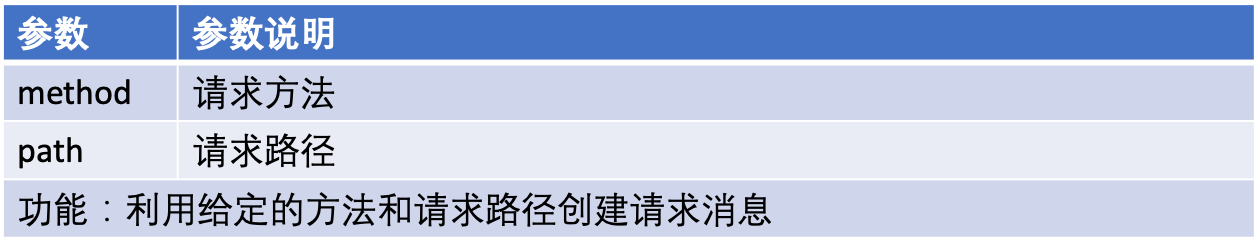
\includegraphics[height = 3.5cm, width = 18cm]{pics/18_Request_table_1_4.png}	
		%\caption{Constructors in BasicHttpRequest}
	\end{figure}

	\begin{lstlisting}[language={java}]
/**
 * Creates request message with the given method, host and request path.
 *
 * @param method request method.
 * @param host request host.
 * @param path request path.
 *
 * @since 5.0
 */
public BasicHttpRequest(final Methods method, final HttpHost host, final String path) {
    super();
    this.method = Args.notNull(method, "Method").name();
    this.scheme = host != null ? host.getSchemeName() : null;
    this.authority = host != null ? new URIAuthority(host) : null;
    this.path = path;
}

	\end{lstlisting}
	\begin{figure}[H]
		\centering
		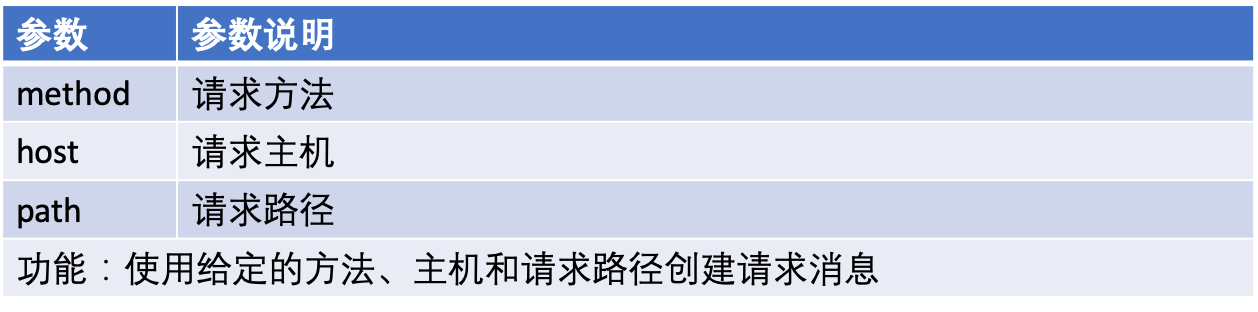
\includegraphics[height = 3.5cm, width = 18cm]{pics/19_Request_table_2_5.png}	
		%\caption{Constructors in BasicHttpRequest}
	\end{figure}

	\begin{lstlisting}[language={java}]
/**
 * Creates request message with the given method, request URI.
 *
 * @param method request method.
 * @param requestUri request URI.
 *
 * @since 5.0
 */
public BasicHttpRequest(final Methods method, final URI requestUri) {
    super();
    this.method = Args.notNull(method, "Method").name();
    setUri(Args.notNull(requestUri, "Request URI"));
}

	\end{lstlisting}
	\begin{figure}[H]
		\centering
		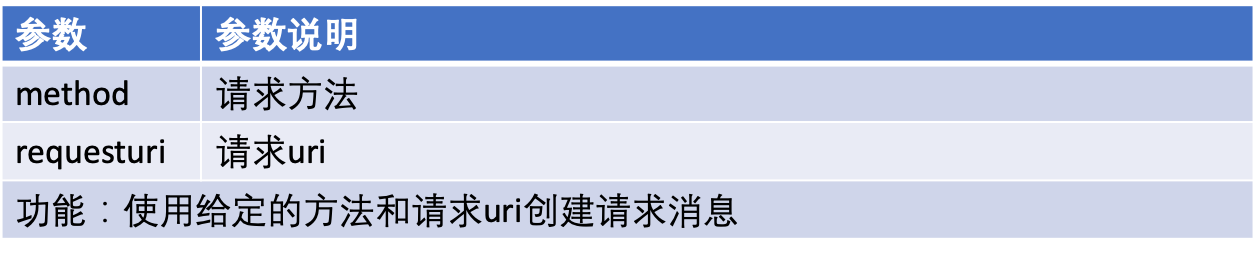
\includegraphics[height = 3.5cm, width = 18cm]{pics/20_Request_table_3_6.png}	
		%\caption{Constructors in BasicHttpRequest}
	\end{figure}

	\subsection{BasicHttpResponse}
	\begin{CJK}{UTF8}{gbsn}
		路径:org.apache.http.message\\
		继承: AbstractHttpMessage\\
		实现接口: HttpResponse
	\end{CJK}{}

	\subsubsection{Methods in BasicHttpResponse}
	\begin{CJK}{UTF8}{gbsn}
		\subparagraph{}
		BasicHttpResponse 中包含了从别的类中继承来的方法,以及其独有的,其关系如 Figure 11 所示。
	\end{CJK}{}
	\begin{figure}[H]
		\centering
		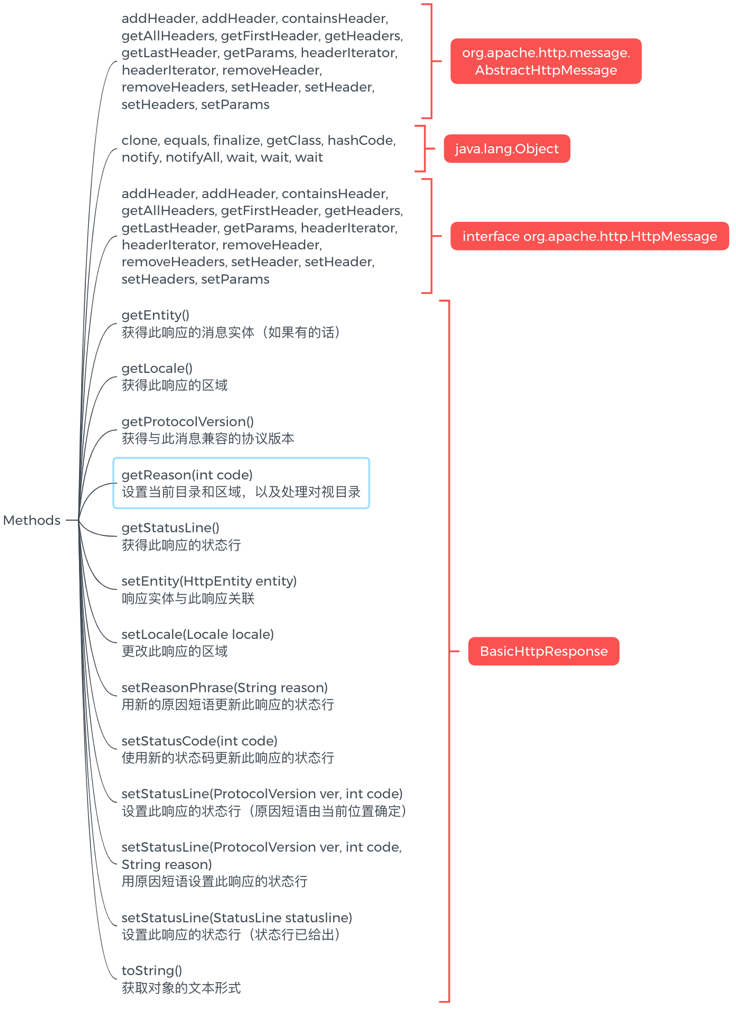
\includegraphics[height = 20cm, width = 16cm]{pics/21_BasicHttpResponse.png}	
		\caption{Methods in BasicHttpRequest}
	\end{figure}

	\subsubsection{Constructors}
	\begin{figure}[H]
		\centering
		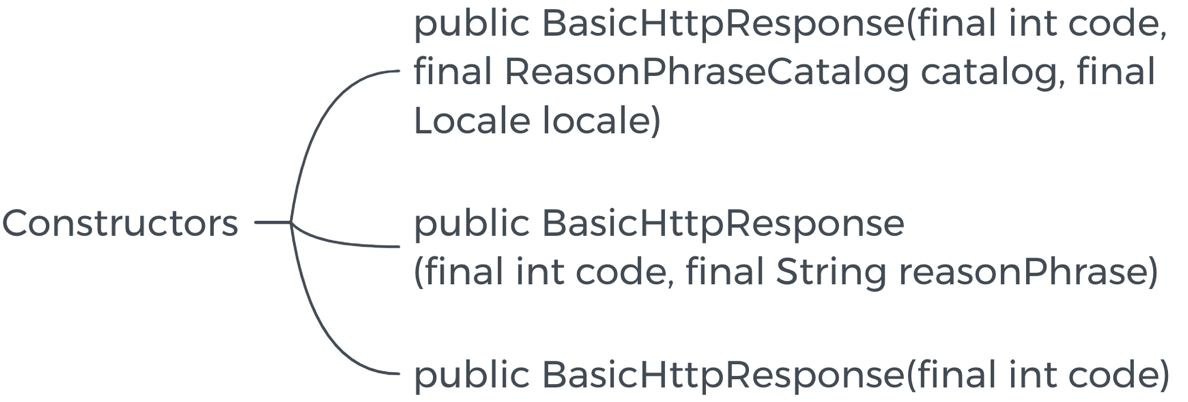
\includegraphics[height = 5cm, width = 14cm]{pics/22_Response_constructors.png}	
		\caption{Constructors in BasicHttpResponse}
	\end{figure}

	\begin{CJK}{UTF8}{gbsn}
		接下来分别介绍 BasicHttpResponse 中的构造器
	\end{CJK}{}

	\hspace*{\fill} \\ %空行

	\begin{lstlisting}[language={java}]
/**
 * Creates a new response.
 *
 * @param code              the status code
 * @param catalog           the reason phrase catalog, or
 *                          {@code null} to disable automatic
 *                          reason phrase lookup
 * @param locale            the locale for looking up reason phrases, or
 *                          {@code null} for the system locale
 */
public BasicHttpResponse(
        final int code,
        final ReasonPhraseCatalog catalog,
        final Locale locale) {
    super();
    this.code = Args.positive(code, "Status code");
    this.reasonCatalog = catalog != null ? catalog : EnglishReasonPhraseCatalog.INSTANCE;
    this.locale = locale;
}
	\end{lstlisting}

	\begin{figure}[H]
		\centering
		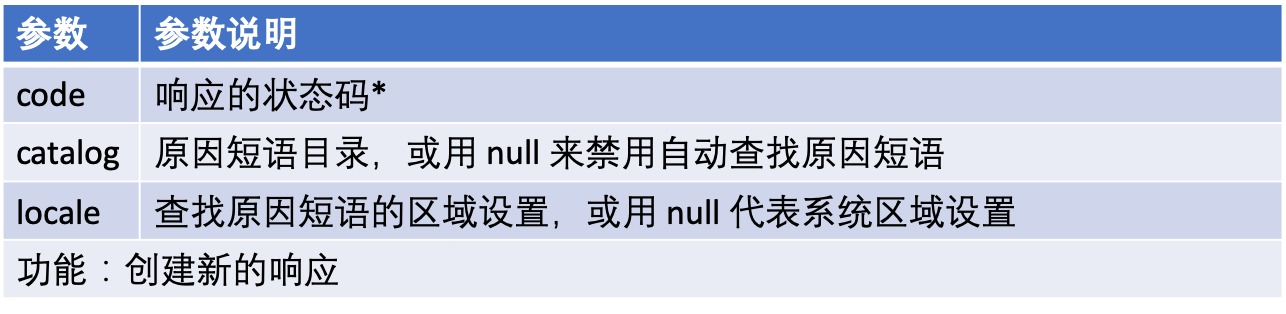
\includegraphics[height = 4cm, width = 18cm]{pics/23_Response_table_1.png}	
		%\caption{Constructors in BasicHttpRequest}
	\end{figure}

	\begin{CJK}{UTF8}{gbsn}
		其中有一个新的概念:status code,状态码,这里介绍一下:
	\end{CJK}{}

	\begin{figure}[H]
		\centering
		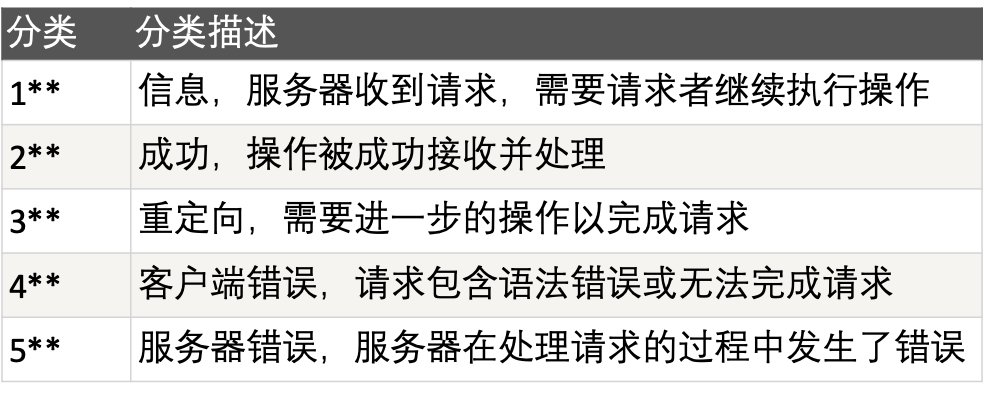
\includegraphics[height = 5.5cm, width = 15cm]{pics/24_status_code.png}	
		\caption{Status Code}
	\end{figure}

	\begin{lstlisting}[language={java}]
/**
 * Creates a new response.
 *
 * @param code          the status code of the response
 * @param reasonPhrase  the reason phrase to the status code, or {@code null}
 */
public BasicHttpResponse(final int code, final String reasonPhrase) {
    this.code = Args.positive(code, "Status code");
    this.reasonPhrase = reasonPhrase;
    this.reasonCatalog = EnglishReasonPhraseCatalog.INSTANCE;
}

	\end{lstlisting}

	\begin{figure}[H]
		\centering
		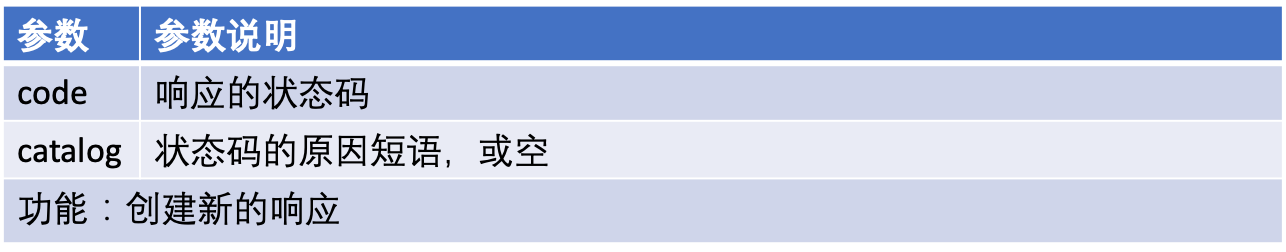
\includegraphics[height = 3.8cm, width = 18cm]{pics/25_Response_table_2.png}	
		%\caption{Constructors in BasicHttpRequest}
	\end{figure}

	\begin{lstlisting}[language={java}]
/**
 * Creates a new response.
 *
 * @param code          the status code of the response
 */
public BasicHttpResponse(final int code) {
    this.code = Args.positive(code, "Status code");
    this.reasonPhrase = null;
    this.reasonCatalog = EnglishReasonPhraseCatalog.INSTANCE;
}

	\end{lstlisting}

	\begin{figure}[H]
		\centering
		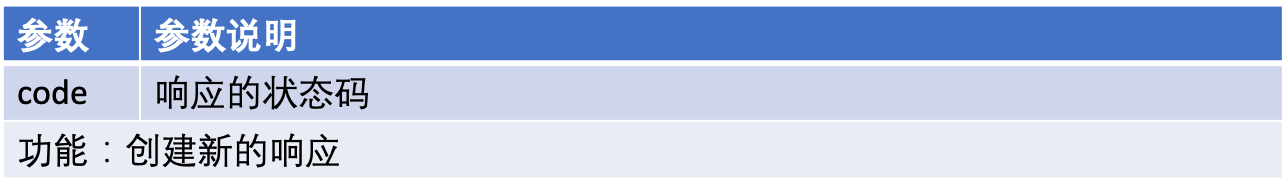
\includegraphics[height = 2.8cm, width = 18cm]{pics/26_Response_table_3.png}	
		%\caption{Constructors in BasicHttpRequest}
	\end{figure}

	\section{Functions}
	\begin{CJK}{UTF8}{gbsn}
		Http请求处理的过程包括以下几个步骤:\\
		\indent 建立连接 (Setting up Connections)\\
		\indent 接收请求 (Receving Requests)\\
		\indent 处理请求 (Processing Requests)\\
		\indent 访问资源 (Accessing Resources)\\
		\indent 构建响应 (Building Response Message)\\
		\indent 发送响应 (Sending out Response)\\
		\hspace*{\fill} \\ %空行
		整个过程如 Figure 14 所示:
	\end{CJK}{}

	\begin{figure}[H]
		\centering
		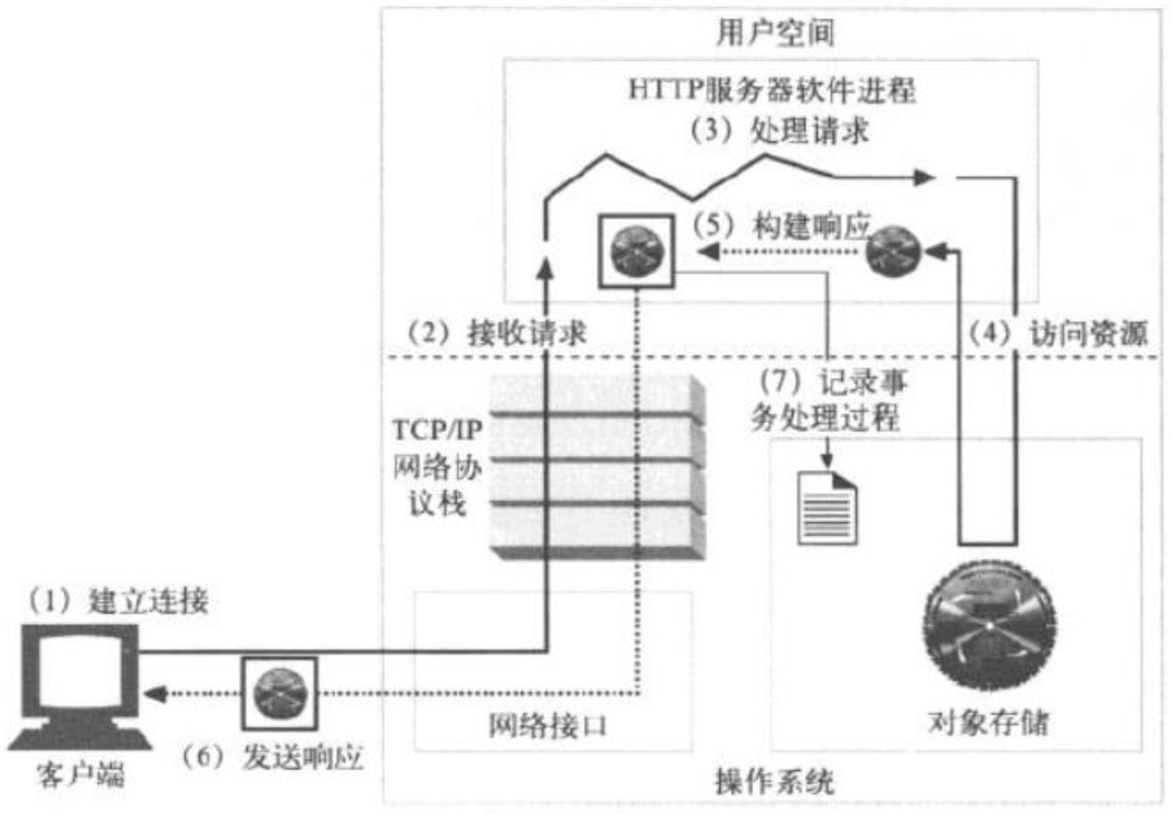
\includegraphics[height = 11cm, width = 16cm]{pics/27_http_procedure.png}	
		\caption{Http Request Processing}
	\end{figure}

	\subsection{Setting up Connections}
	\begin{CJK}{UTF8}{gbsn}
		建立连接之前先要进行域名解析(把域名指向网站空间IP,DNS服务器把域名解析到IP地址)。\\
		建立连接:接收或拒绝连接请求
	\end{CJK}{}

	\subsection{Receving Requests}
	\begin{CJK}{UTF8}{gbsn}
		HTTP请求报文:由请求行(request line)、请求头部(header)、空行和请求数据4个部分组成,如 Figure 15 所示。\\ 
		接收请求:接收客户端请求报文中对某资源的请求。
	\end{CJK}{}

	\begin{figure}[H]
		\centering
		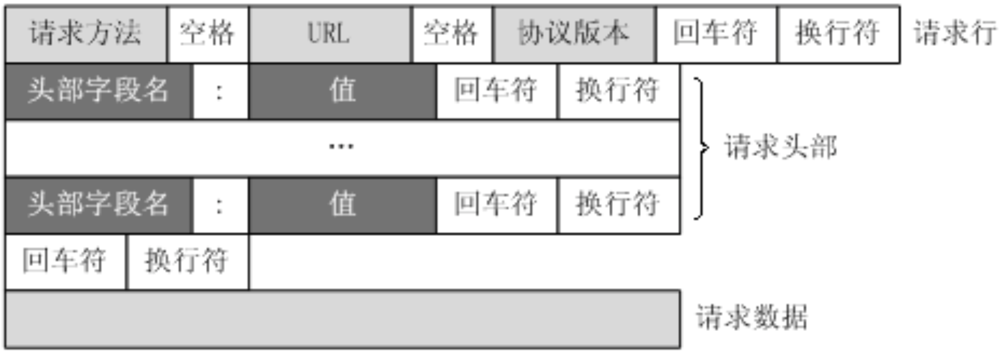
\includegraphics[height = 5cm, width = 14cm]{pics/28_request_format.png}	
		\caption{Request Format}
	\end{figure}

	\subsection{Processing Requests}
	\begin{CJK}{UTF8}{gbsn}
		\subparagraph{}
		处理请求:服务器对请求报文进行解析,获取请求的资源及请求方法等相关信息 根据方法,资源,首部和可选的主体部分对请求进行处理。\\
		(之前说过,http常用的请求方法:GET 、 POST 、 PUT 、 DELETE 、 PATCH、HEAD、OPTIONS、TRACE、\\
		CONNECT)
	\end{CJK}{}

	\subsection{Accessing Resources}
	\indent 
	\begin{CJK}{UTF8}{gbsn}
		%\subparagraph{}
		\indent 访问资源:服务器获取请求报文中请求的资源web服务器(存放了web资源的服务器),负责向请求者提供对方请求的静态资源或动态运行后生成的资源。\\
		%\subparagraph{}
		\indent 如果请求静态资源,客户端发起询问上一次修改到现在之间有没有再修改。若返回状态码为服务器端没修改(304),浏览器会直接读取本地的该资源的缓存文件(负载均衡)。如 Figure 16 所示,可以看到第二次访问同一对象的时候直接从 cache 里面拿数据。
	\end{CJK}{}

	\begin{comment}
	\begin{figure}
		\centering
		\subfigure[The First Access]{
			\begin{minipage}[H]{0.5\textwidth}
				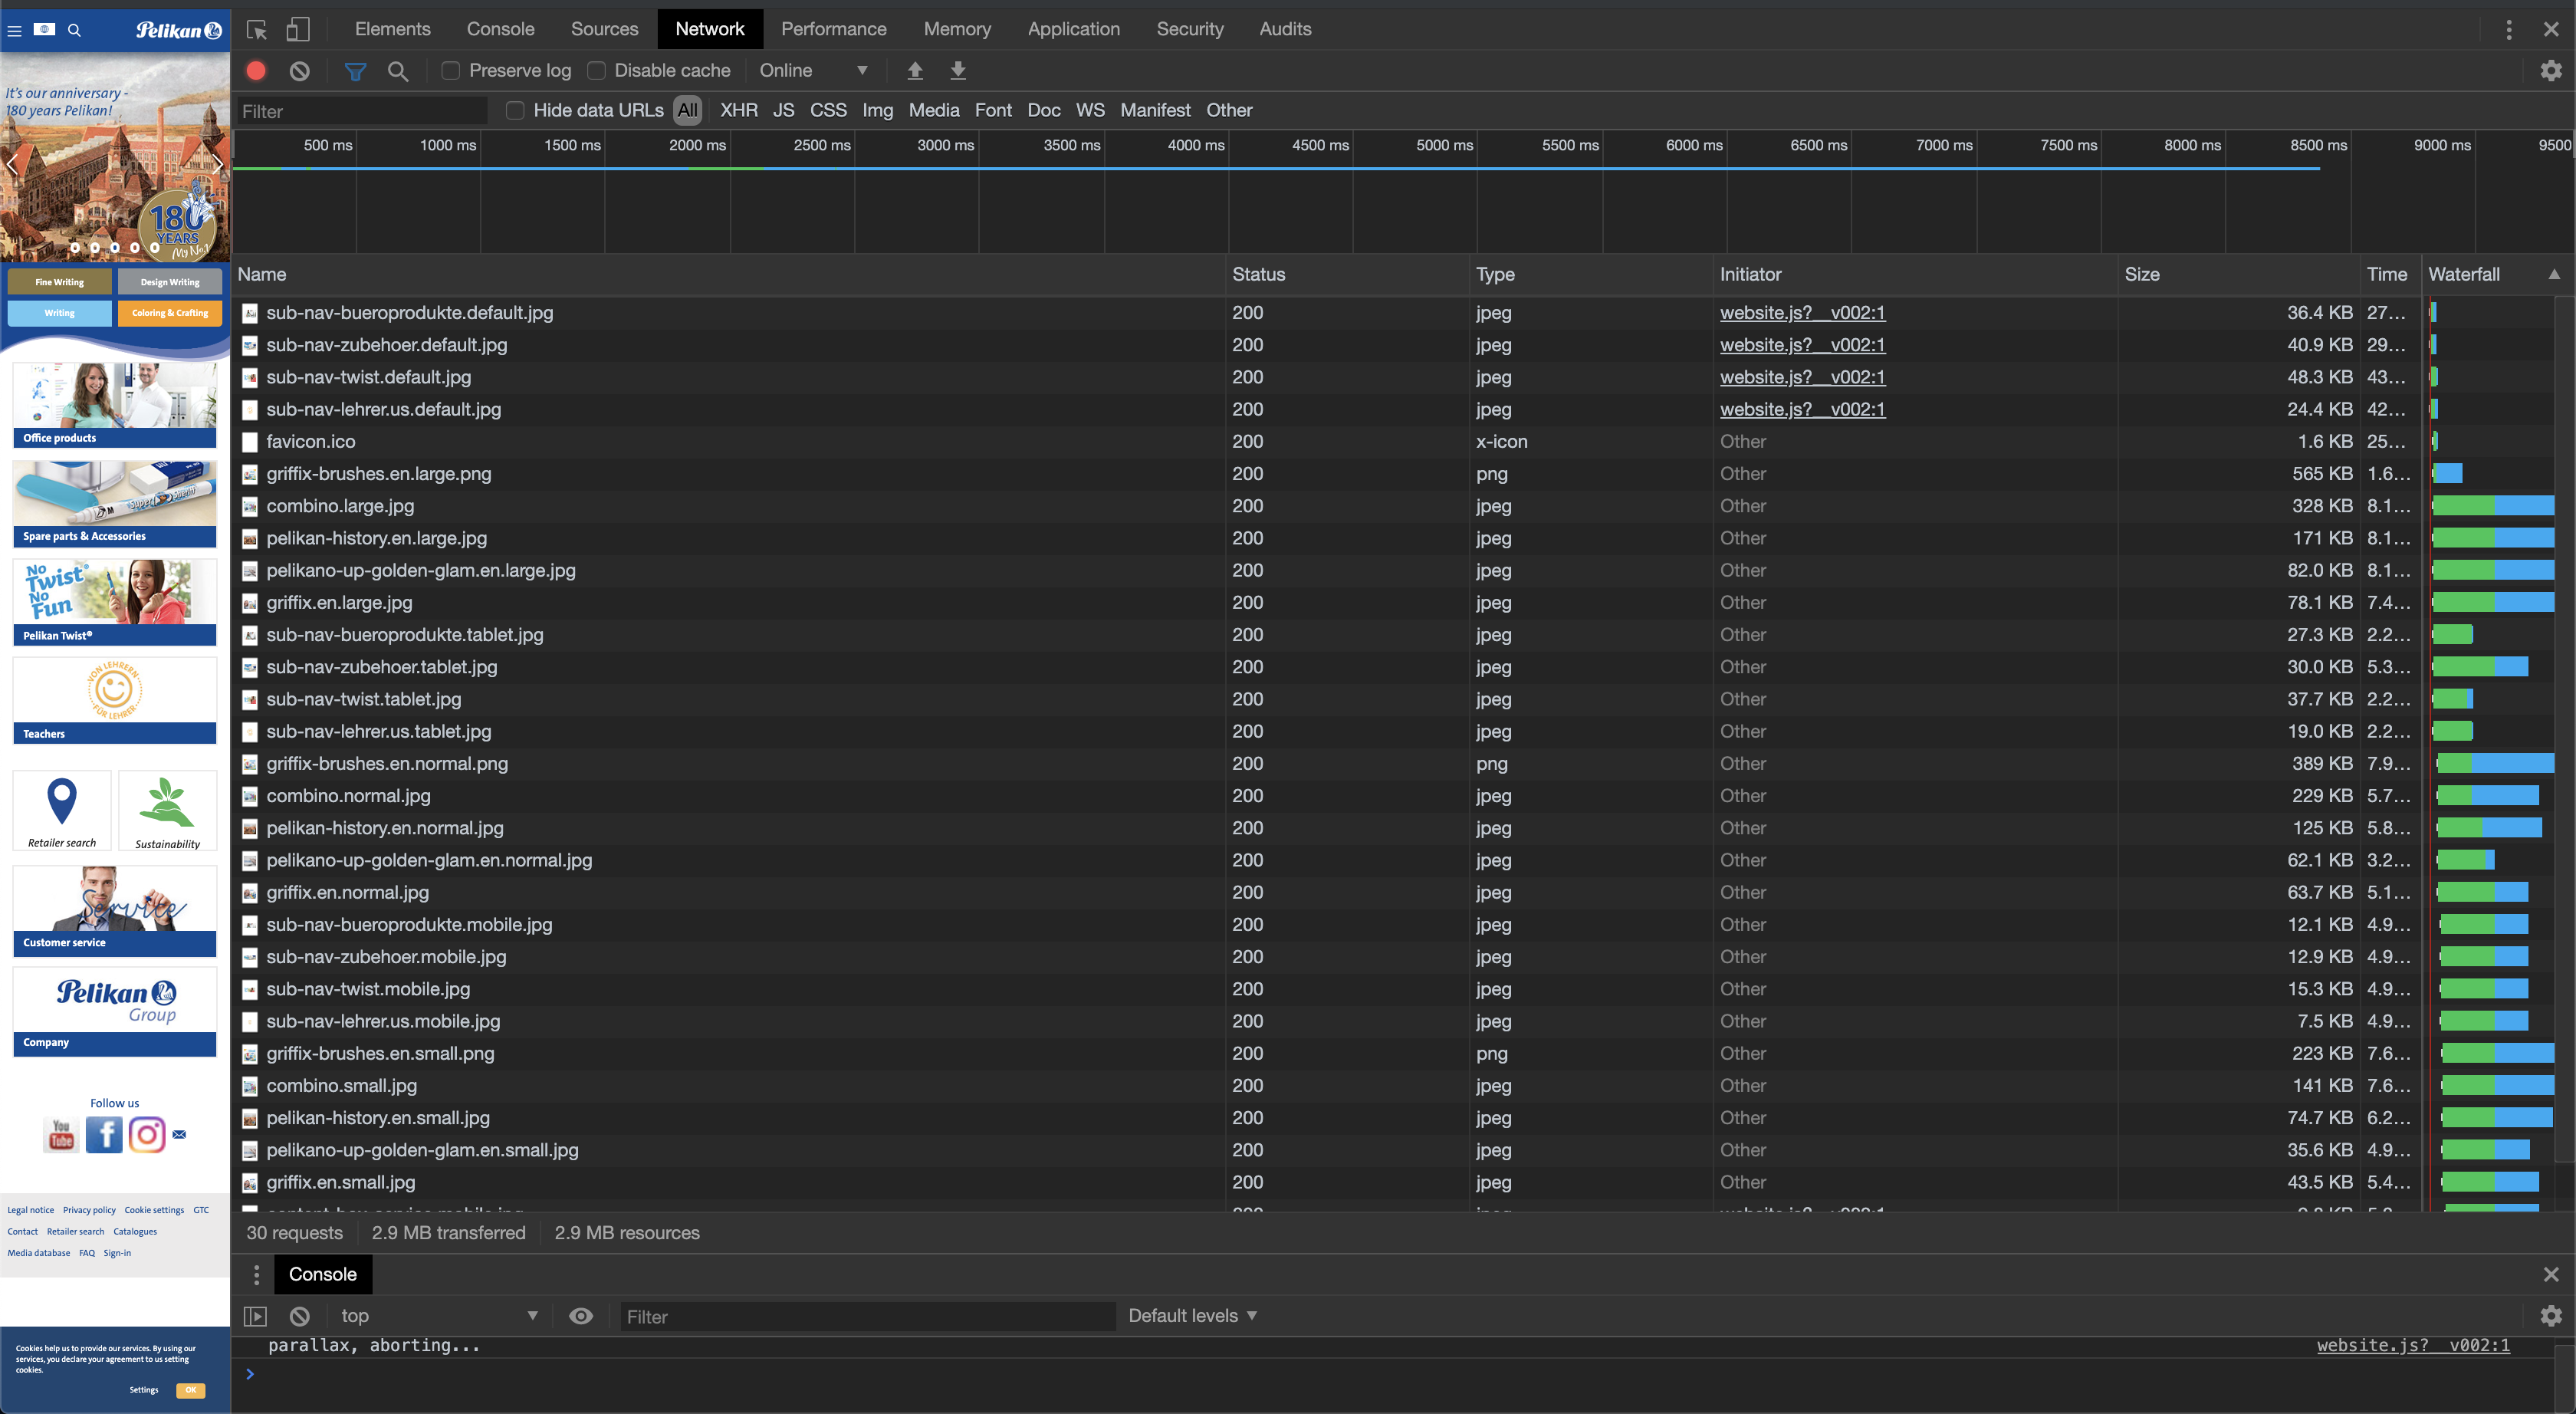
\includegraphics[width=1\textwidth]{pics/29_first_access.png}
			\end{minipage}
		}
		\subfigure[The Second Access]{
			\begin{minipage}[H]{0.5\textwidth}
				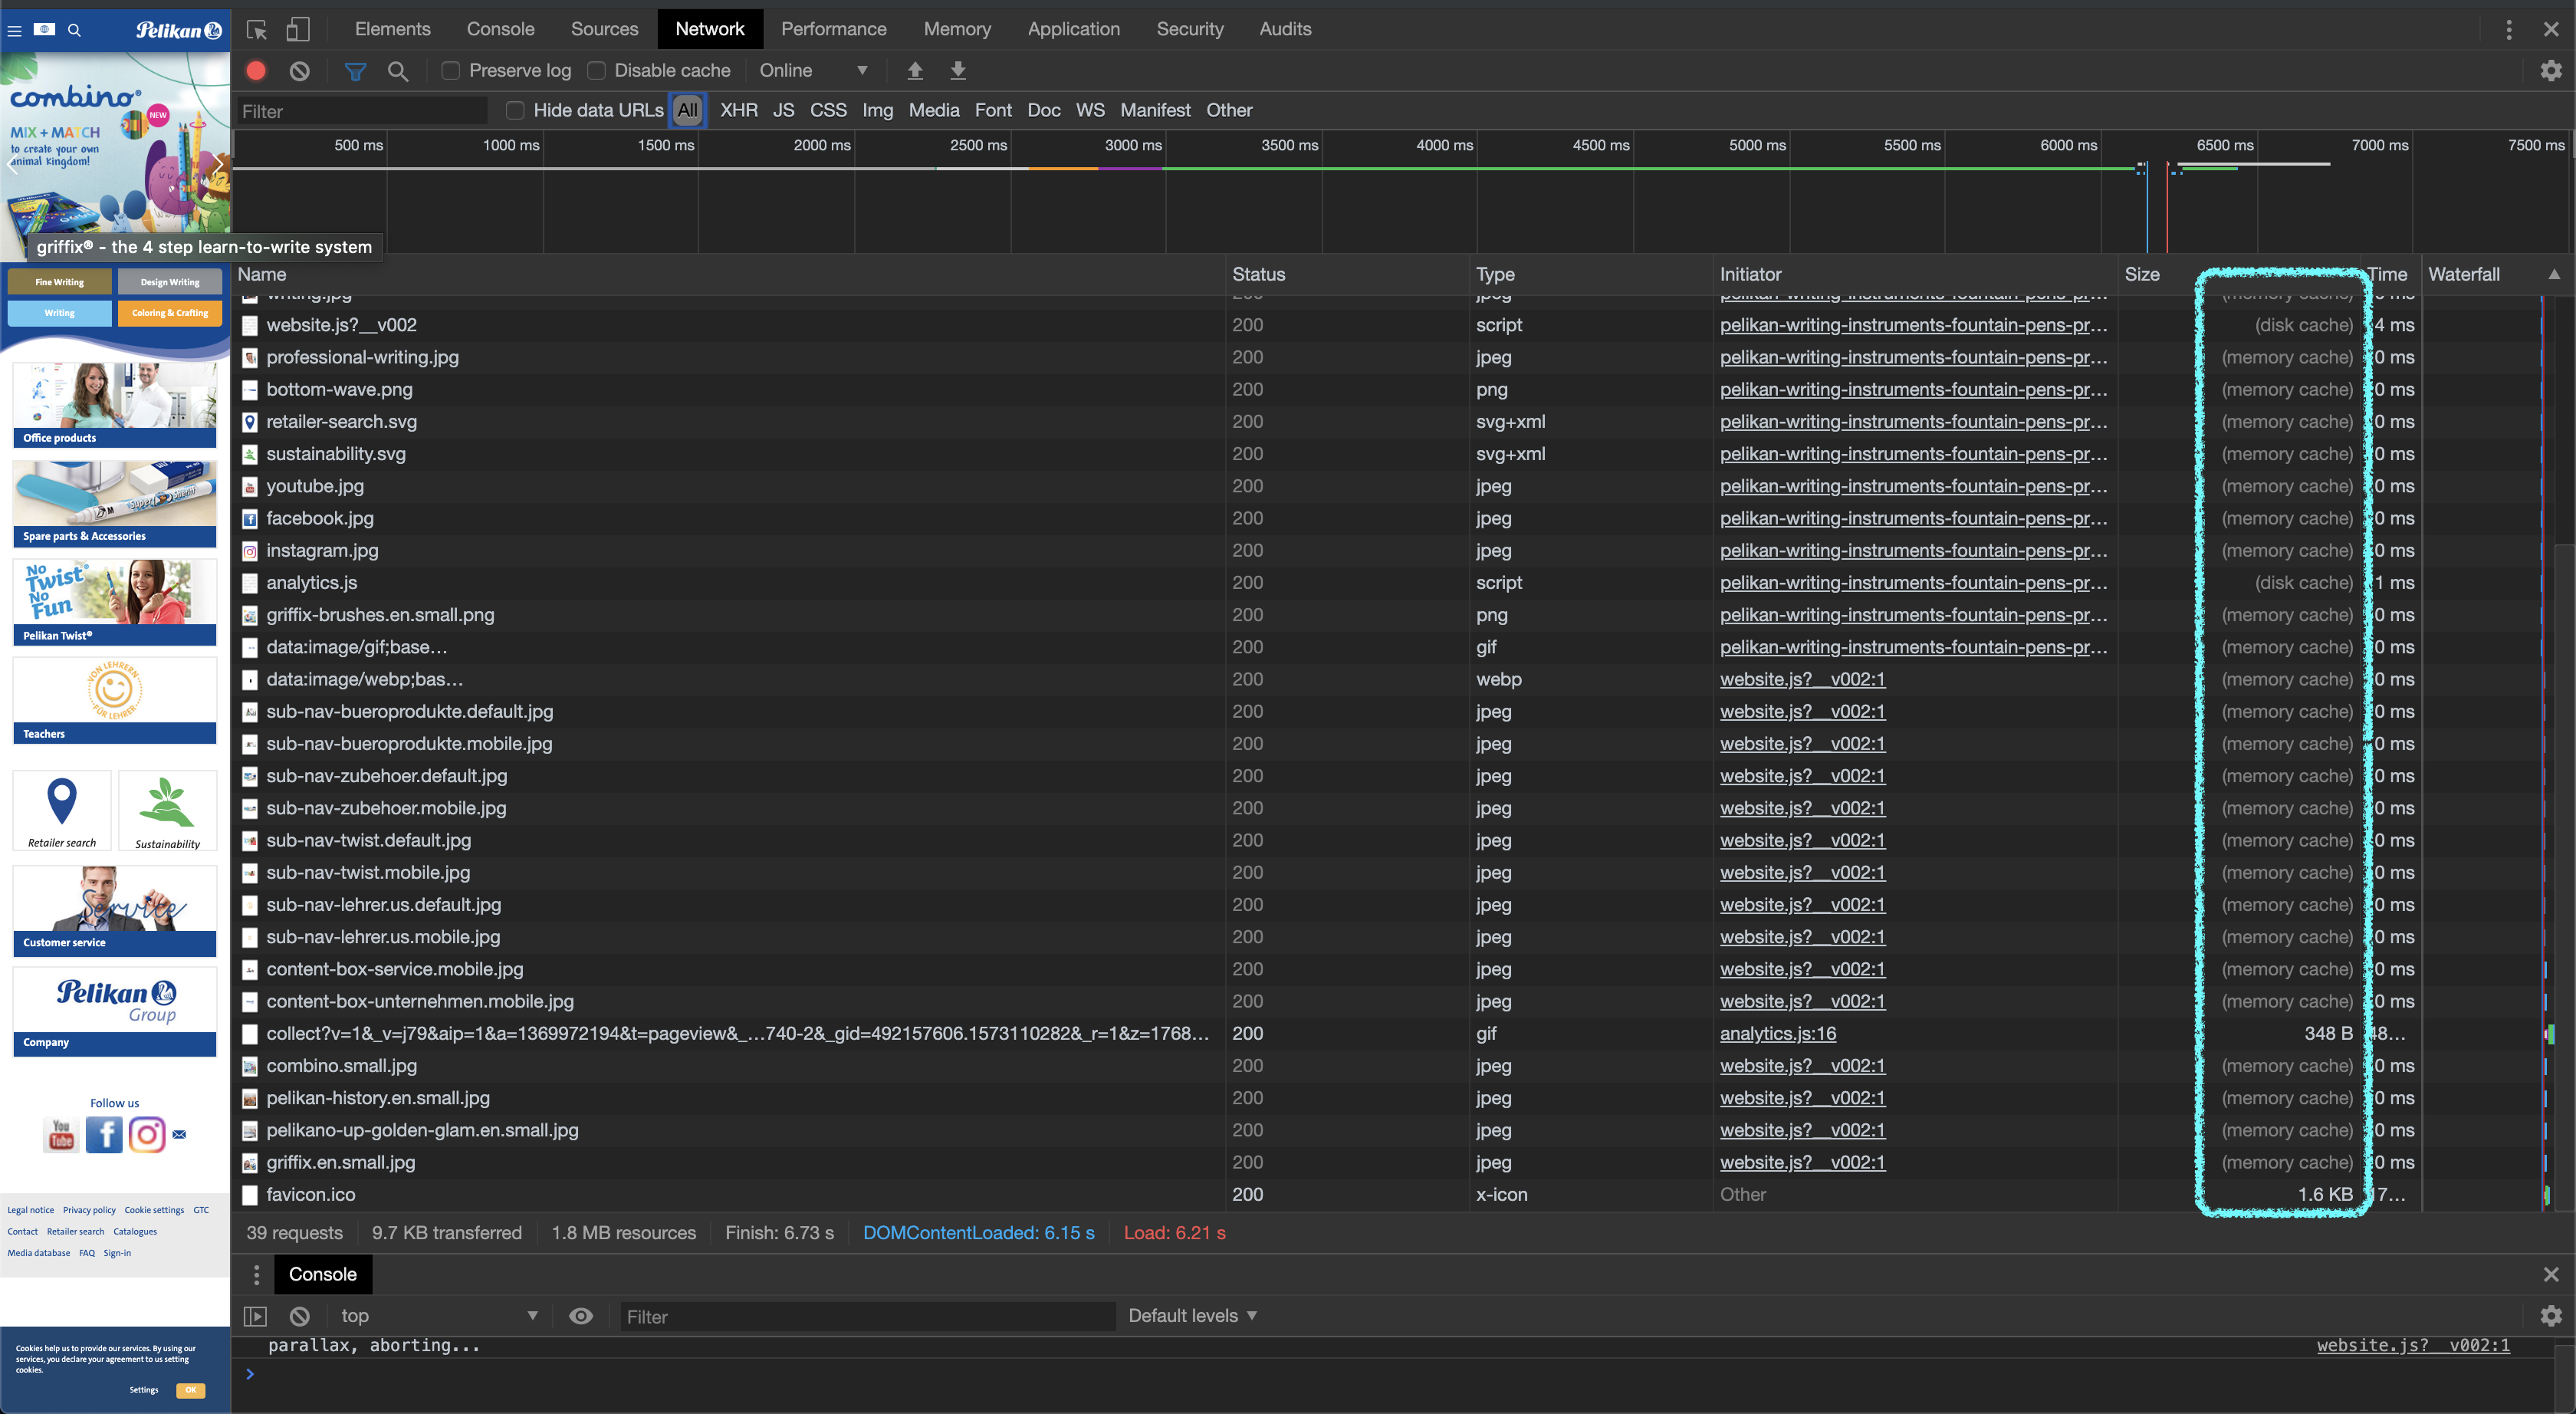
\includegraphics[width=1\textwidth]{pics/30_second_access.png}
			\end{minipage}
		}
		%\caption{大标题} \label{fig:1}
	\end{figure}
	\end{comment}

	\begin{figure}[htbp]
	\centering    %居中
	\subfigure[The First Access] {
		\begin{minipage}[H]{19cm}
			\centering          %子图居中
			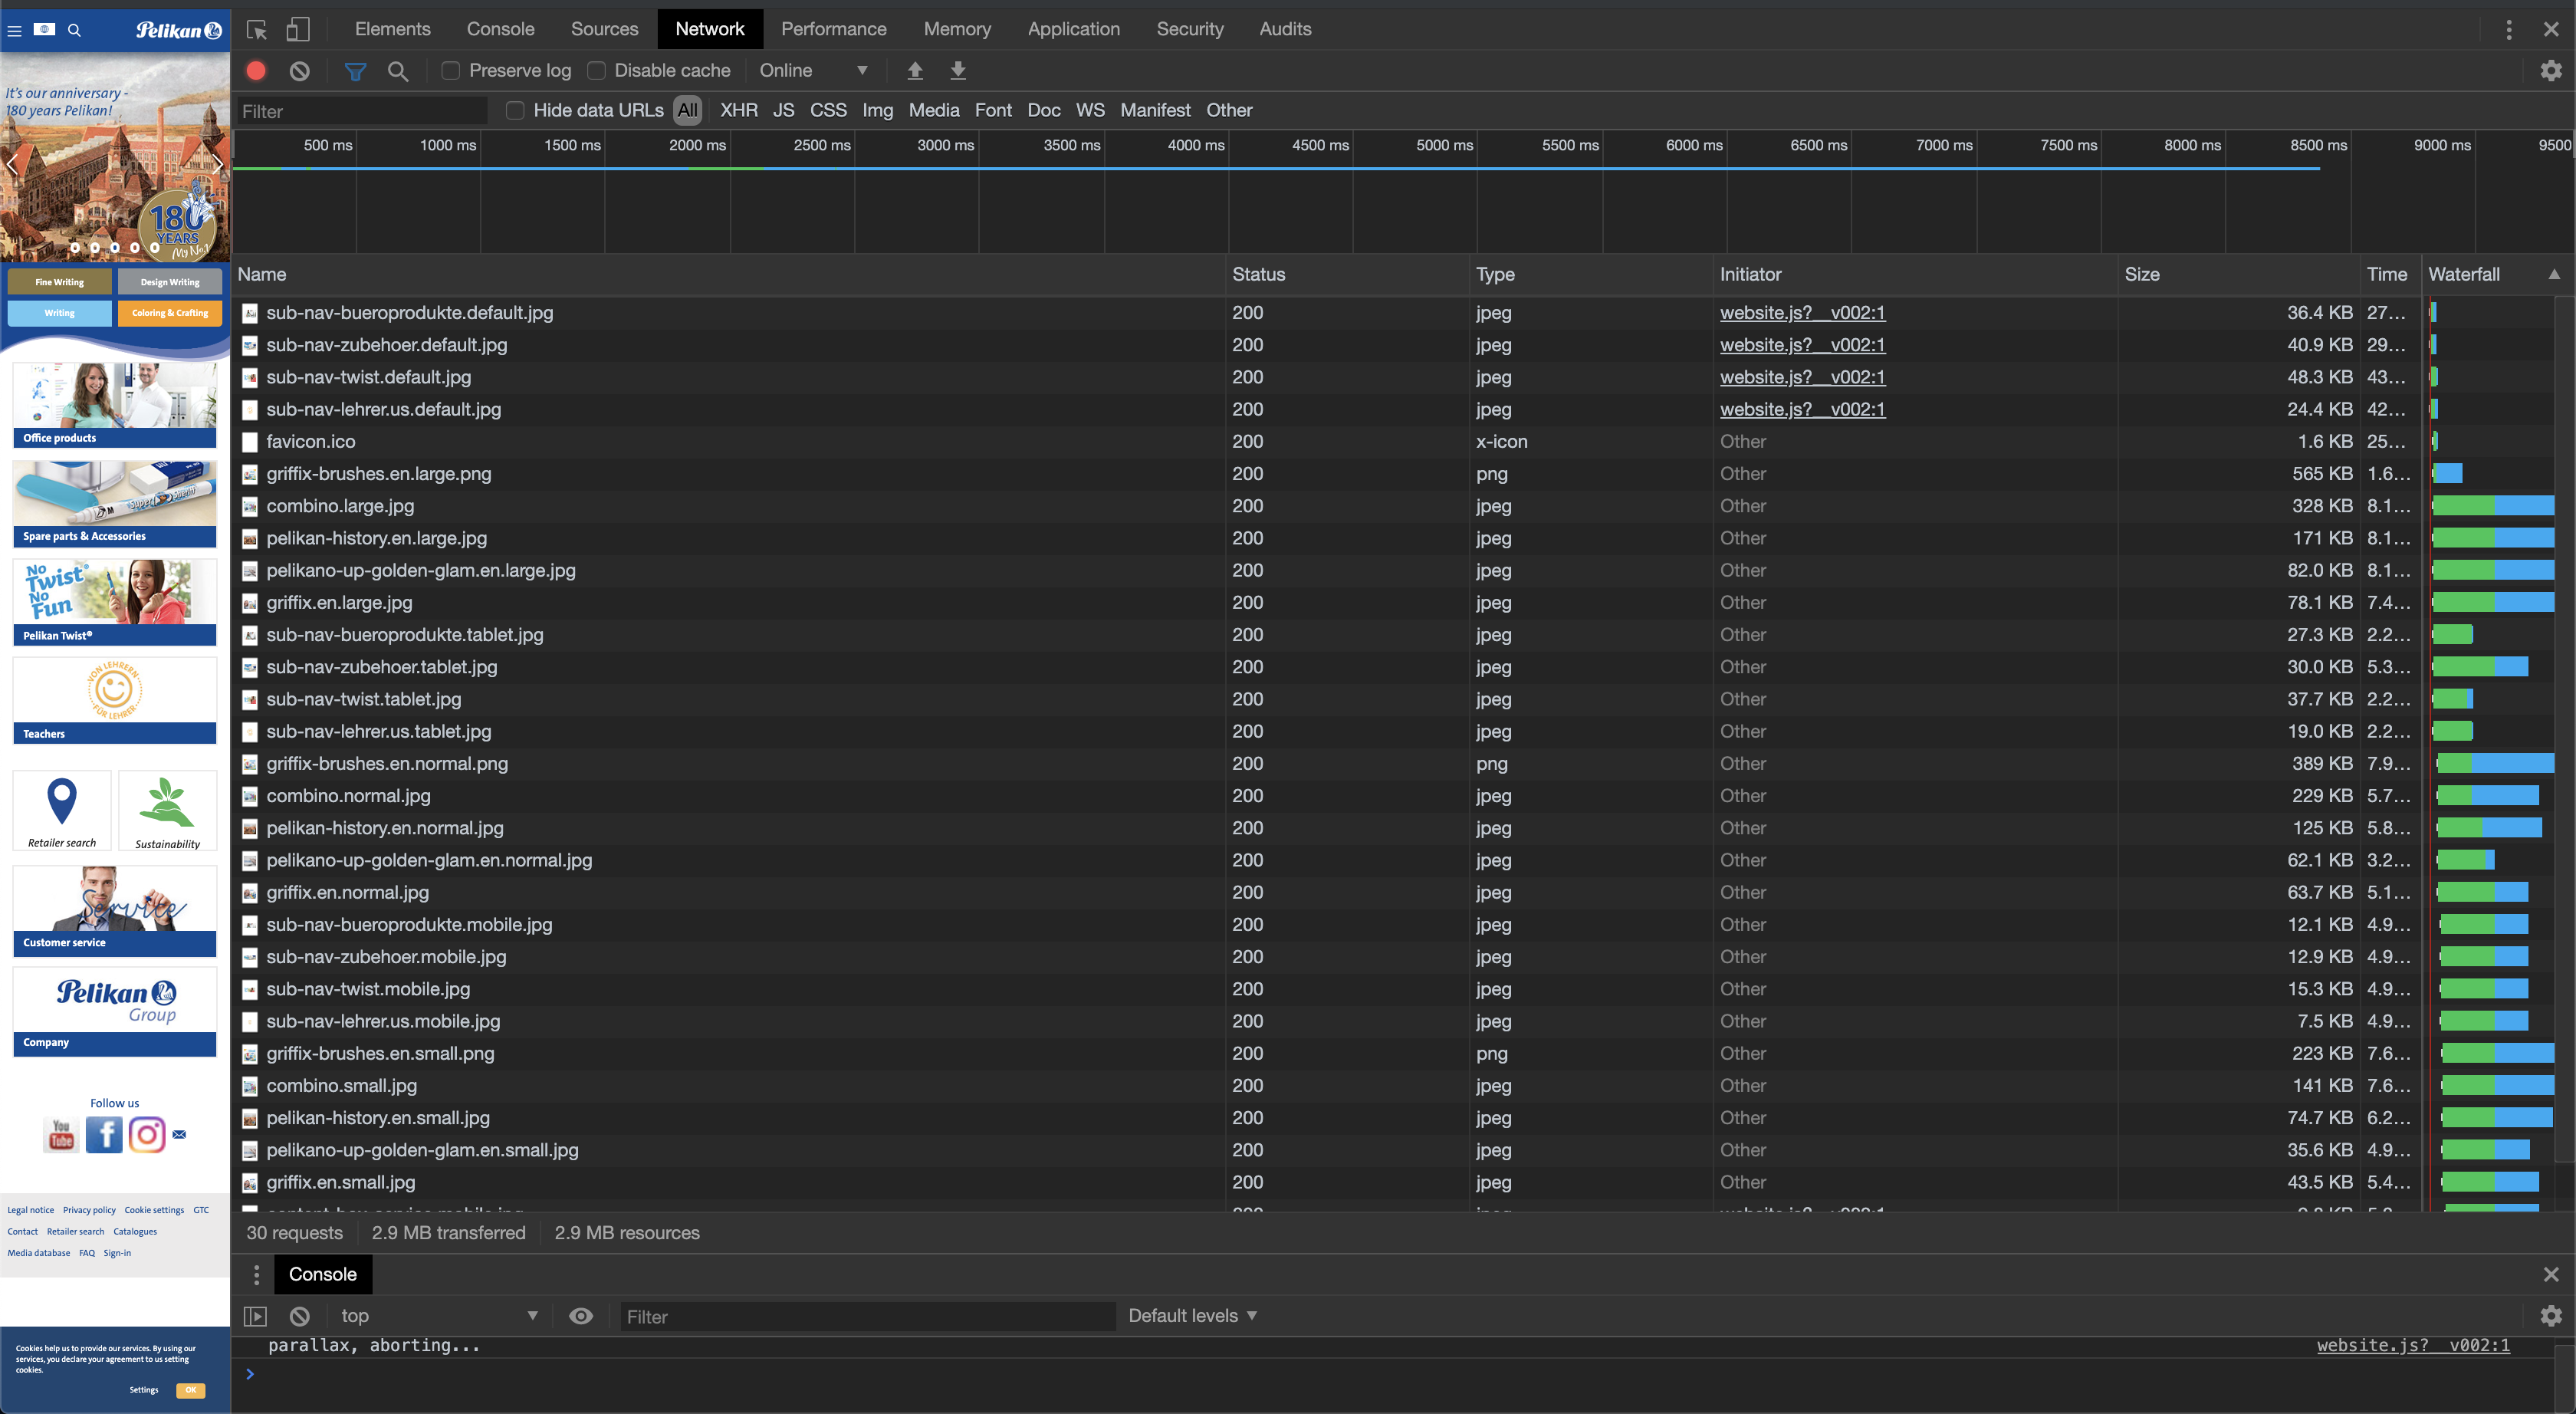
\includegraphics[scale = 0.22]{pics/29_first_access.png}   %以pic.jpg的0.5倍大小输出
		\end{minipage}
	}
		
	\subfigure[The Second Access] {
		\begin{minipage}[H]{19cm}
			\centering      %子图居中
			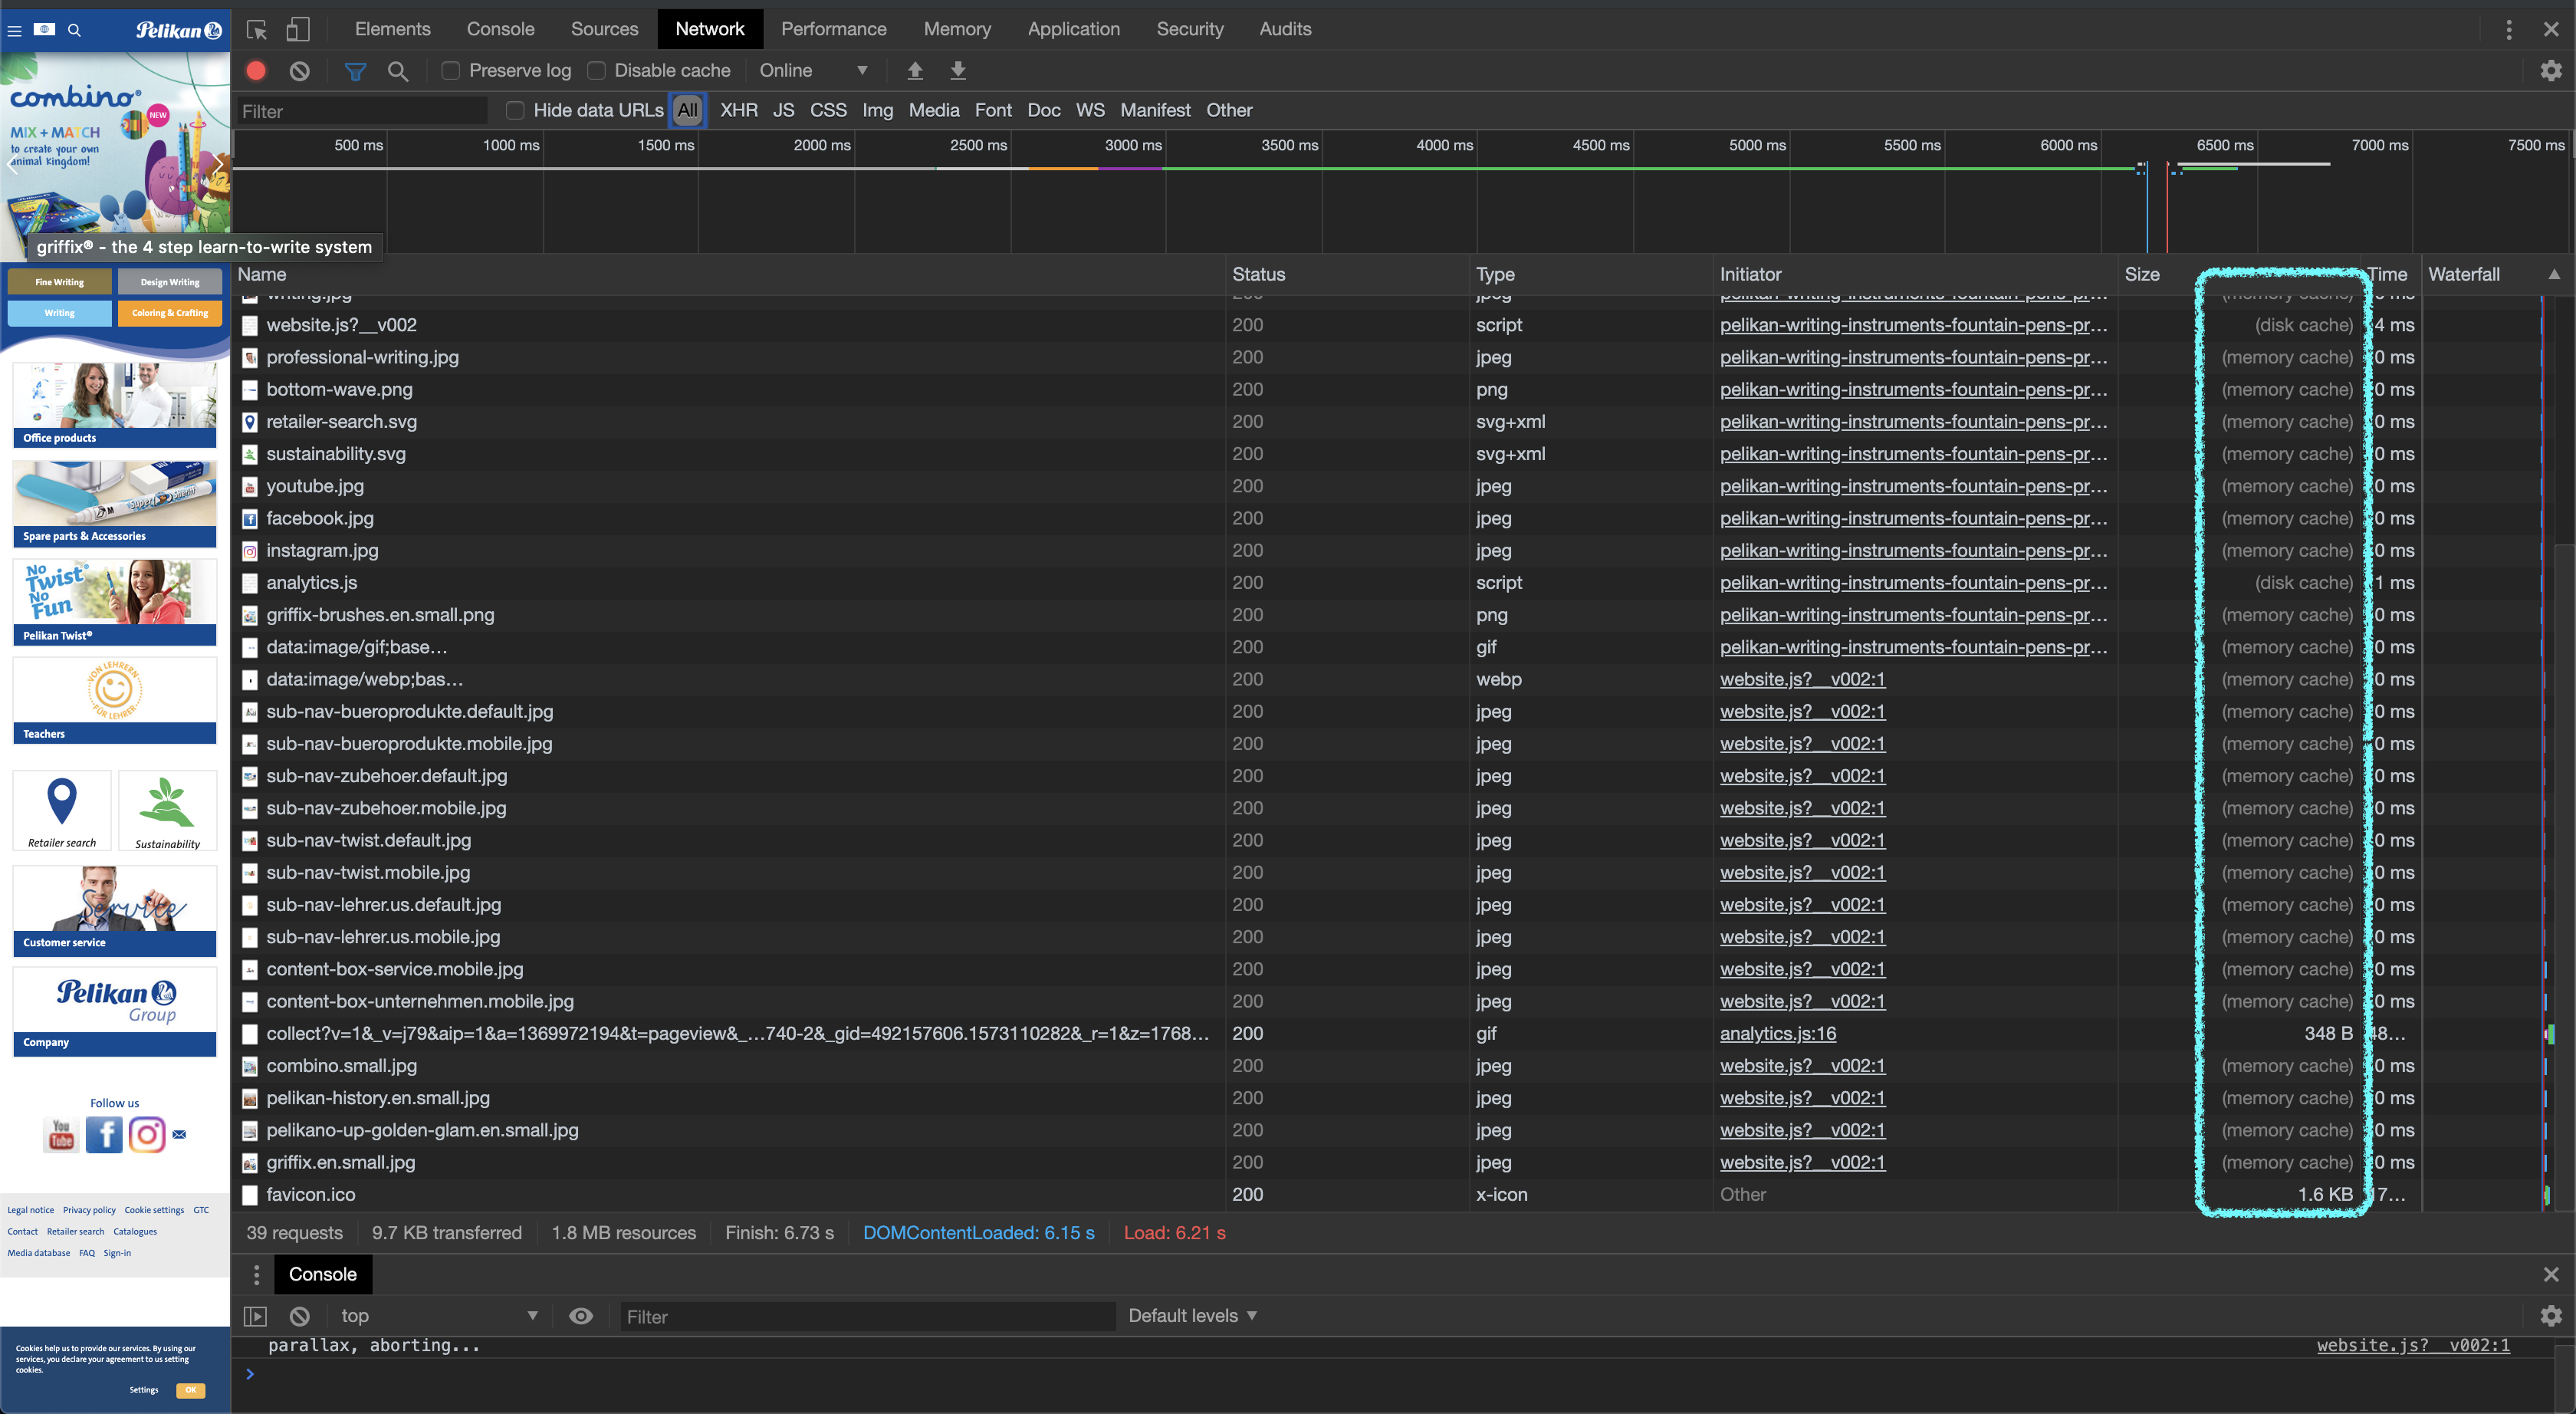
\includegraphics[scale = 0.22]{pics/30_second_access.png}   %以pic.jpg的0.5倍大小输出
		\end{minipage}
	}
	 
	\caption{Two Visits} %  %大图名称
	\label{fig:1}  %图片引用标记
	\end{figure}

	\clearpage

	\subsection{Building Response Message}
	\begin{CJK}{UTF8}{gbsn}
		\subparagraph{}
		构建响应报文:一旦Web服务器识别除了资源,就执行请求方法中描述的动作,并返回响应报文。响应报文中包含有响应状态码、响应首部,如果生成了响应主体的话,还包括响应主体。
	\end{CJK}{}

	\clearpage
%%%%%%%%%%%%%%%%%%%%%%%%%%%%%%%%%% NEW PAGE %%%%%%%%%%%%%%%%%%%%%%%%%%%%%%%%%%%%%%%%%


\end{document}